\documentclass[11pt, titlepage]{report}
\usepackage[utf8]{inputenc}
\usepackage[T1]{fontenc}
\usepackage{hyperref} % für BiblaTex
\usepackage{listings} % für Listen / Quellcode-Ausschnitte
\usepackage{siunitx} % für Einheiten (Ohm etc.)
\usepackage[left=3cm, right=2.5cm, top=3cm, bottom=2cm]{geometry}
\usepackage{hsellogo}
\usepackage{hselfonts}
\usepackage{hselcolor}
\usepackage{hselmath}
\usepackage{parskip}
\usepackage{csquotes} %für BiblaTex
\usepackage{acronym} % für Abkürzungsverzeichnis
\usepackage{subcaption} % für Bildunterschriften mit a und b
\usepackage{microtype} % für Optik der Lesbarkeit
\usepackage{lmodern} % behebt Probleme mit der Schriftgröße der Fußnoten
\usepackage{booktabs}
\usepackage{pdfpages}
\usepackage{lscape} % für Querformat
\usepackage[ngerman, german]{babel}
\usepackage[citestyle=science,bibstyle=numeric, sorting = none,
hyperref=true,backref=true,maxcitenames=3,url=true,backend=biber,natbib=true]{biblatex}
\addbibresource{references.bib}
\author{Liebenow,Tino}
\date{\textit{<2020-01-26 Sun>}}
%Verminderung von Trennstrichen bei Zeilenumbrüchen:
\tolerance=1
\emergencystretch=14em %\maxdimen für nohyphen
\hyphenpenalty=100 % 10000 für nohyphen
\hbadness=10000

\begin{document}
	\begin{titlepage}
	\hsellogo\hfill Projektarbeit
	\par
	\vspace{4cm}
	\noindent\parbox{0.8\textwidth}{\Huge RotaCon - Dokumentation}  
	\vspace{2cm}


	\Large \noindent vorgelegt von:
	\begin{itemize}
		\item Tino Liebenow - Matrikelnummer 7011830
	\end{itemize}
	\vspace{2cm}
	betreut duch\newline
	Dipl.-Ing. (FH) Jörg Strick\newline
	Abgabedatum: 05.03.2020
	\end{titlepage}
	\newpage
	\noindent E I D E S S T A T T L I C H E \hspace{1em} V E R S I C H E R U N G

		Ich, der/die Unterzeichnende, erkläre hiermit an Eides statt, dass ich die vorliegende Arbeit selbständig verfasst habe und keine anderen als die angegebenen Quellen und Hilfsmittel benutzt habe. Alle Quellenangaben und Zitate sind richtig und vollständig wiedergegeben und in den jeweiligen Kapiteln und im Literaturverzeichnis wiedergegeben. Die vorliegende Arbeit wurde nicht in dieser oder einer ähnlichen Form ganz oder in Teilen zur Erlangung eines akademischen Abschlussgrades oder einer anderen Prüfungsleistung eingereicht.  Mir ist bekannt, dass falsche Angaben im Zusammenhang mit dieser Erklärung strafrechtlich verfolgt werden können.

		\vspace{50pt}
		\noindent\rule{5cm}{.4pt}\hfill\rule{5cm}{.4pt}\par
		\noindent Datum, Ort \hfill Unterschrift
	\newpage
	\tableofcontents
	\newpage
	\begingroup
		\renewcommand\clearpage{\relax}
		\listoffigures
		\listoftables
	\endgroup
	\newpage
    \section*{\Huge Abkürzungsverzeichnis}% Abkürzungen
    \label{sec:Abkürzungsverzeichnis}
    \vspace{1cm}
	\begin{acronym}
		\acro{ad}[A/D]{Analog / Digital}
		\acro{cad}[CAD]{computer-aided design}
		\acro{dsub}[D-Sub]{D-Subminiatur, eine Bauform für ein Steckersystem}
		\acro{eeprom}[EEPROM]{electrically erasable programmable read-only memory}
		\acro{eq}[EQ]{Equalizer}
		\acro{hsel}[HSEL]{Hochschule Emden Leer}
		\acro{ide}[IDE]{Integrated Development Environment}
		\acro{io}[I/O]{Input / Output}
		\acro{ir}[IR]{Infrarot}
		\acro{lcd}[LCD]{liquid crystal display}
		\acro{tp}[TP]{Tiefpass}
		\acro{usb}[USB]{Universal Serial Bus}
    \end{acronym}
	\newpage
	\chapter{Überblick}
		Viele medientechnische Geräte, zum Beispiel Aktivlautsprecher haben ihren Lautstärkeregler an der Rückseite. Zur Bedienung ist der Nutzer somit gezwungen sich unmittelbar am Gerät zu befinden. Von dieser Position ist die Beurteilung der gewählten Einstellungen jedoch eher ungenau und erfordert häufig eine weitere Person zur Unterstützung. Der RotaCon soll dem Abhilfe verschaffen und eine alleinige Bedienung optimieren. Diese Dokumentation beschreibt die Entwicklung des Gerätes und ist in fünf Hauptteile gegliedert. Im ersten Kapitel wird die Ausgangssituation geschildert, sowie die Kerngedanken zum RotaCon. Folgend sind diese Gedanken zu einem Konzept geformt und kategorisch aufgeteilt im zweiten Kapitel niedergeschrieben. Das dritte Kapitel bildet den inhaltlichen Hauptteil der Dokumentation und erläutert die Entwicklung des RotaCon-Prototyps, gefolgt von einer kurzen Zusammenfassung und schlussendlich den Anhängen. Das gesamte Projekt ist als GitHub-Repository mit all seinen Bestandteilen öffentlich einsehbar\footnote{GitHub-Repository: \protect\href{https://github.com/derTino89/RotaCon}{github.com/derTino89/RotaCon}}. 
		\newline Aus Gründen der Lesbarkeit wird in dieser Arbeit die männliche Form für Personenbeschreibungen genutzt.
		Diese beziehen sich trotzdem auf Angehörige aller Geschlechter/Gender.
	\section*{Ziel}
		Ziel ist es ein Gerät zur Fernbedienbarkeit von Potentiometern, speziell an Lautsprechern, zu entwickeln. Dabei sollen weder Veränderungen am Lautsprechergehäuse, noch an der Technik vorgenommen werden. Zusätzlich ist eine Diskretisierung der Pegelwerte und deren Visualisierung via LCD-Display angedacht, sodass der Benutzer sichtbare 
		Werte zur Orientierung der aktuellen Einstellung bekommt. 
	\section*{Stand der Technik}	
		Fernsteuerungen für Pegeleinstellungen sind nicht neu auf dem Markt. Dabei sind zwei Varianten verbreitet, zum einen besteht die Möglichkeit, den Potentiometer auf der Platine des Lautsprechers auszutauschen, zum Anderen die Integrierung eines Controllers in den Signalweg. Die erste Variante setzt somit die Öffnung des Lautsprechergehäuses sowie Manipulation der Elektronik voraus. Dies ist nicht nur für den durchschnittlichen
		Lautsprecherbesitzer ein schwieriger Eingriff, sondern hat ebenfalls Einfluss auf diverse Garantieansprüche. Die andere Variante beinhaltet keine Veränderungen am Lautsprecher selbst, regelt jedoch nur die Signalpegel zum Lautsprecher hin und nicht den integrierten Verstärker. Somit muss für diese Version der Verstärker stets auf Maximum geregelt sein, dies hat je nach Verstärker\footnote{Der Stromverbrauch von Klasse A Verstärkern wird aufgrund des konstanten Ruhestroms nicht beeinflusst.} Einflüsse auf Soundqualität und Stromverbrauch.
	\chapter{Konzeptentwurf}
		Das folgende Kapitel beinhaltet die theoretischen Bestandteile zur Umsetzung der Idee. Diese bilden in ihrer Gesamtheit das Konzept,
		nachdem der Prototyp entwickelt wird.
		\section{Theorie Hardware}
		\label{sec:Theorie Hardware}
			Lautstärkeregler sind in den meisten Fällen Potentiometer oder Inkrementalgeber. Diese besitzen in der Regel eine 6mm oder 6.35mm Achse, in D-Form oder geriffelt. Um diese Achse rotieren zu können muss also ein Motor mit einer passenden Kupplung angebracht werden. Für präzise Kontrolle und ausreichendes Drehmoment ist ein Schrittmotor geeignet. Diesen gibt es in verschiedenen Ausfertigungen: unipolar und bipolar. 
			\newline Unipolare Schrittmotoren haben vier Phasen (Elektromagnete) und werden nur in einer Richtung von Strom durchflossen. Bipolare polen ihre Magnetfelder durch Umkehrung der Stromrichtung um, sie haben zwei Phasen, erreichen ein höheres Drehmoment und sind durch ihre Funktionsweise etwas aufwendiger anzusteuern [Schrittmotoren \cite[S.4]{Schrittmotoren}]\footnote{Angaben in eckigen Klammern sind verweise auf das Literaturverzeichnis [Bezeichnung(Referenznummer,Seite)]}.
			\newline Für eine Schrittmotorsteuerung sind drei Funktionseinheiten notwendig. Diese bestehen aus Mikrocontroller, Steuerschaltung und Treiberstufen. Für dieses Projekt ist ein unipolarer Schrittmotor ausreichend, da keine hohen Drehmomente erreicht werden müssen. Dies hat zusätzlich den Vorteil, dass die Steuerschaltung simpel ist und rein auf Softwarebasis gelegt werden kann. Als Treiber soll eine Darlington-Schaltung für den Motor dienen. Die softwaretechnische Steuerung ist durch ein Arduino mit integriertem Mikrocontroller angestrebt, dessen Spannungsversorgung von 5V idealer Weise auch für die anderen Komponenten ausreichen soll, sodass ein Betrieb des Gerätes durch USB-Spannungsversorgung ermöglicht wird. 
			\newline Da analoge Drehregler durch eine Minimal- und Maximalstellung begrenzt sind, ist auch der Antrieb des Motors in diesen Bereichen zu stoppen. In erster Linie sollen Endschalter den Potentiometer-Anschlag erkennen und Software-gesteuert die Rotation einstellen. Redundant dazu wird der Stromverbrauch des Schrittmotors durch die Kombination eines nicht-invertierenden Verstärkers und dem Analog-Digital-Wandler vom Mikrocontroller überwacht. 
			\newline Für die Bedienung des Gerätes soll ein Infrarotempfänger mit passender Fernbedienung im Frequenzbereich verwendet werden. Da sich Lautstärkeregler meist nicht sichtbar am Lautsprecher befinden, ein IR-Empfänger jedoch eine quasioptische Verbindung voraussetzt, bieten sich zwei getrennte Gehäuseteile an, die durch ein Kabel verbunden sind. In dem sichtbaren Gehäuse befindet sich zusätzlich das Display.
		\newpage
		\section{Theorie Software}
		\label{sec:Theorie Software}
			Softwaretechnisch sind drei Bereiche in diesem Projekt abzudecken:
			\begin{enumerate}
				\item Programmierung des Mikrocontrollers
				\item Entwurf von Schaltung und Platinenlayout
				\item Modellierung der Gehäuse
			\end{enumerate} 

			Bei der Programmierung des Mikrocontrollers soll beachtet werden, dass die aktuellen Werte der Motorstellung und der dazugehörigen Lautstärkeanzeige gespeichert werden, damit bei jeder Inbetriebnahme die jeweils vorherigen Werte beibehalten bleiben. Die einzige Schnittstelle zum Benutzer ist das Display, daher müssen Fehler, Warnungen und wichtige Informationen auf dem Display abgebildet werden. Alle variablen Funktionen des Gerätes sollen über die Fernbedienung steuerbar sein, also die Steuerung der Lautstärke, aber auch das Aktivieren, bzw. Deaktivieren der Displaybeleuchtung.

			Für den Entwurf der Schaltung sowie die Erstellung des Platinenlayouts soll ein Leiterplatten-Editor benutzt werden. So können externe Platinen-Hersteller oder hochschuleigene Maschinen die Produktion der Leiterplatten sicherstellen.

			Die Gestaltung der Gehäuse muss präzise modelliert werden, damit Steckverbindungen und Display formschlüssig integriert werden können. Dabei soll zusätzlich darauf geachtet werden, dass alle Teile von einem 3D-Drucker gefertigt werden können.


		\section{Theorie Mechanik und Design}
		\label{sec:Design}
			Die Übertragung des Drehmoments vom Motor an den Drehregler des Lautsprechers kann nur stattfinden, wenn der Motor starr gelagert ist. Daher ist das Gehäuse mit Motor und Motorsteuerung zu fixieren. Weiterhin sind Lautstärkeregler an unterschiedlichen Lautsprechern auch an verschiedenen Positionen, sodass dieses Gehäuse zusätzlich in seiner Position variabel positionierbar sein muss. 
			\newline Einige Lautsprecher mit stärkeren Verstärkern haben zusätzlich Kühlkörper an der Rückseite des Lautsprechers. Aus diesem Grund und der Tatsache, dass eventuell weitere Regler (Phase, TP, EQ)\footnote{Phasenverschiebung, Grenzfrequenz des Tiefpass-Filters, Equalizer.} vorhanden sind, ist ein gewisser Abstand zwischen den Gehäusen notwendig. Auch die Positionen der Endanschläge sind nicht überall gleich, das bedeutet, dass auch die Endschalter in ihrer Position variierbar sein müssen.
			\newline Aufgrund der Komplexität der Gehäuse-Voraussetzungen wird der Schwerpunkt beim Prototyp auf die mechanische Funktionalität gelegt, sodass das Design nach Abschluss der Funktionstests angepasst und optimiert werden kann.
		\label{sec:Theorie Mechanik}
	\chapter{Prototyp-Entwicklung}
	\label{sec:Praxistil}
		Folgendes Kapitel beinhaltet die Beschreibung aller im RotaCon verwendeten Bestandteile, sowie der Software, die zum Entwickeln benutzt wurden.
		Es wird auf die Programmierung des Mikrocontrollers eingegangen, die elektronische Schaltung und der Entwurf der Gehäuse wird erläutert.
		\section{Notwendige Software}
			Die folgend näher erläuterten Programme wurden bei der Entwicklung des RotaCon verwendet und sind keine zwingende Voraussetzung zur Produktion. Jedes dieser Programme kann bei Bedarf durch äquivalente Software ersetzt werden. 
			\subsection*{Arduino IDE}
			\label{sec:Arduino IDE}
				%gleiche Quellen wie oben
				Diese Entwicklungsumgebung (IDE\footnote{IDE steht für \textit{Integrated Development Environment} und bedeutet Entwicklungsumgebung.}) stellt den Softwareteil der Arduino-Plattform dar und basiert auf Processing, einer stark typisierten Programmiersprache mit integrierter Entwicklungsumgebung. Die Programmiersprache ähnelt C++ und ist darauf ausgelegt, ohne tiefgründige Programmierkenntnisse Programme schreiben zu können. Programme dieser IDE werden ''Sketch'' genannt. \newline Solch ein Sketch wird in der Umgebung kompiliert und kann via USB-Schnittstelle direkt auf den Speicher des Arduino-Boards geladen werden. Ein in die IDE integrierter serieller Monitor kann die jeweiligen Zustände der Ein- und Ausgänge überwachen und ist ein Hilfsmittel zur Fehlersuche in der Entwicklungsphase.
				\newline Damit die Übertragung des Sketches stattfinden kann, muss jedoch vorerst das richtige Board mit dem richtigen Prozessor in den Werkzeugen ausgewählt werden. Verwendete Version: Arduino 1.8.10
			\subsection*{FreeCAD}
			\label{sec:FreeCAD}
				FreeCAD\footnote{CAD steht für \textit{computer-aided design} und beschreibt das rechnergestützte Erzeugen geometrischer Modelle.} ist eine parametrische Modellierungsanwendung. 3D-Objekte können mit hoher Präzision modelliert und angeordnet werden. Vorteil gegenüber einer Modellierungsanwendung, wie Cinema 4D, besteht in der Möglichkeit der Herstellung von Unterlagen zum designten Modell. So können beispielsweise technische Zeichnungen und Montagepläne erstellt werden. [FreeCAD\cite{FreeCAD}] 
				\newline Die Anwendung ist ein Open-Source-Projekt, daher wird es gemeinschaftlich weiterentwickelt und wächst in seinem Funktionsumfang. Verwendete Version: FreeCAD 0.18
				%https://www.freecadweb.org/wiki/Getting_started/de
				%https://de.wikipedia.org/wiki/CAD#Herstellen_von_Fertigungs-/Herstellungsunterlagen
			\newpage	
			\subsection*{Cura}
			\label{sec:Cura}
				%https://de.wikipedia.org/wiki/Slicer-Software
				%https://ultimaker.com/download/170/Cura_User-Manual_v1.0.pdf
				Cura ist eine Slicing Software der Firma Ultimaker. Dieses Programm ist für die Umwandlung von 3D-Objektmodellen in spezifische Druckanweisungen verantwortlich. Dazu wird ein 3D-Modell zu einem Stapel von flachen Schichten umgerechnet beziehungsweise ''zerschnitten''. Zusätzliche Einstellungen für den 3D-Drucker werden vorgegeben, sodass Druckablauf, Temperaturen von Druckbett und Extruder, Filament-Art, 
				Vortriebsgeschwindigkeiten und gegebenenfalls Stützen für den Druck von Überhängen festgelegt sind. [Cura User-Manual\cite[S.26-29]{Cura}]
			\subsection*{Eagle}
			\label{sec:Eagle}
				%http://dl36mmdz94630.cloudfront.net/uploads/eagle_resources/files/000/002/278/original/step-by-step_tutorial.pdf?1484967932
				Die Software Eagle von Autodesk ist ein Platinen-CAD Programm zum Entwerfen von Schaltplänen und Platinenlayouts.[Eagle \cite{Eagle}] Dabei sind zwei Hauptschritte der Bearbeitung auszuführen. Zum einen die Gestaltung des Schaltplans, wobei Eagle durch Einbinden von Bibliotheken annähernd alle erdenklichen Schaltsymbole und Bezeichnungen darstellen kann, die für den Entwurf der Schaltung notwendig sind. Zusätzlich können manuell Symbole erstellt werden, falls spezielle unkonventionelle oder eigens entwickelte Elemente verwendet werden.
				Im zweiten Schritt wird das Layout der Platine entworfen, um die Leiterbahnen und Bohrungen passend zu platzieren beziehungsweise zu dimensionieren.
		\section{Verwendete Hardware}
				\subsection*{Arduino Nano}
				\label{sec:Nano}
					%Arduino Praxiseinstieg 2.3 Seite 23?
					%https://store.arduino.cc/arduino-nano
					%Bild: http://www.circuitstoday.com/arduino-nano-tutorial-pinout-schematics
					Arduino ist eine Open-Source Elektronik Plattform, die aus zwei Teilen besteht. Einem Hardware- und einem Softwareteil [Brühlmann \cite[S.23]{Arduino_Plattform}]. Der Hardware-Teil ist eine Mikrocontroller-Schaltung mit serieller Schnittstelle. Diese ''Mikrocontroller-Boards'' gibt es in verschiedenen Ausführungen und unterscheiden sich in ihrer Größe, dem verwendeten Mikrocontroller und den somit einhergehenden Eigenschaften von Ein- und Ausgängen. Die Eingänge können Daten von Sensoren einlesen, die Ausgänge dienen zur Ansteuerung von Motoren, Dioden,	Relais oder anderen elektronischen Komponenten. Die Spannungsversorgung kann über die USB-Schnittstelle oder externem Netzteil erfolgen. 
					\newline Der im RotaCon verwendete Arduino Nano ist eine Leiterplattenversion von geringer Baugröße und nutzt als Basis den ATmega328 [Arduino \cite{Nano}]. Der Arduino Nano hat insgesamt 22 Input/Output-Pins, 8 davon können als analoge Eingänge benutzt werden. Die logische Spannung des Nanos beträgt 5V, die maximale Stromstärke pro Pin 40 mA. Mit einer Taktrate von 16 MHz und einem integrierten Speicher (EEPROM) von 1KB ist der Arduino Nano wegen seinen Funktionen für dieses Projekt gewählt worden.
					
					\begin{figure}[htbp]
						\centering
						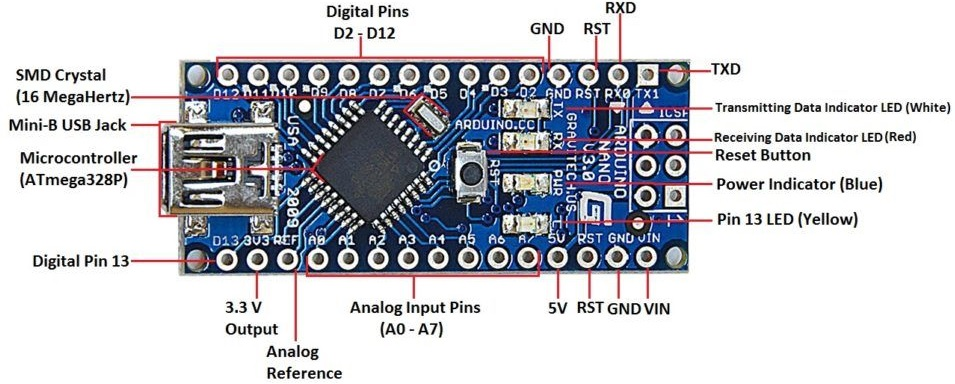
\includegraphics[width=0.8\linewidth]{./img/Nano_PinOut.jpg}
						\caption[Übersicht Arduino Nano]{ Übersicht Arduino Nano [Bildquelle: \cite{NanoImg}]
						\label{fig:imgNano}}
					\end{figure}
			\newpage
			\subsection*{Schrittmotor (unipolar)}
			\label{sec:Motor}
				%Fachkunde Elektrotechnik Seite 461
				%http://home.roboticlab.eu/de/examples/motor/stepper
				%http://www.arduino-projekte.de/index.php?n=63
				Der im RotaCon verwendete unipolare Schrittmotor \textit{28BYJ-48} hat vier Phasen. Das bedeutet vier Elektromagneten steuern die Bewegung des Dauermagnetrotors. Diese vier Elektromagneten werden durch zwei Spulen realisiert, deren Wicklungen je hälftig aufgeteilt und entgegengesetzt gewickelt sind. Sie sind statisch um den Rotor (Anker) angeordnet. Die einzelnen Phasen werden nur in einer Richtung von Strom durchflossen und steuern so die Polung der Magneten beziehungsweise die Rotationsrichtung des Motors. 
				\newline Die Versorgungsspannung beträgt 5V und der Widerstand einer Spule ist mit 50$\Omega$ +- 7\% angegeben. Je nach Einphasensteuerung\footnote{Es wird genau eine Halbspule geschaltet.} oder Zweiphasensteuerung\footnote{Es werden zwei benachbarte Halbspulen geschaltet, die nicht Teil der gleichen Induktivität sind.} ergeben sich daher unterschiedliche Ströme. Da die Spannungsversorgung des Motors je zwischen den Halbspulen anliegt (vergl. Abb.\ref{fig:Spulen}) und sie somit parallel geschaltet sind, ist der Gesamtwiderstand bei Zweiphasensteuerung nur halb so groß (12,5$\Omega$). 
				\newline Bei Schrittmotoren werden im Datenblatt Schrittwinkel und Getriebeübersetzung angegeben. Der hier verwendete Motor hat einen Schrittwinkel von 5,625° bei 64 Schritten angegeben und ein Getriebeverhältnis von 1/64. Daraus ergibt sich, dass eine volle Umdrehung der Motorachse 4096 Schritte benötigt (64x64). Diese Winkelangabe bezieht sich auf einen Halbschrittbetrieb, daher ist im Vollschrittbetrieb der Schrittwinkel 11,25° und eine Achsenumdrehung benötigt 2048 Schritte [vergl. Tkotz et al. \cite[S.641]{Winkelberechnung}]. Bei einem Halbschrittverfahren werden Ein- und Zweiphasensteuerung zusammen benutzt, um den Motor in 45° Schritten zu bewegen [vergl. Deltron AG \cite[S.7]{Schrittmotor_Steuerung}] 
				\newline Die Verwendung eines unipolaren Motors hat den Vorteil, dass aufgrund der einseitigen Stromflussrichtung, die Steuerung rein durch Software erfolgen kann und daher auf H-Brücken oder ähnliche zusätzliche Schutzmaßnahmen in diesem Projekt verzichtet werden kann.


				\begin{equation}
					\label{eq:StromMinMax}
					I=\frac{U}{R}=\frac{5V}{25\Omega} = 200mA \hspace{20pt} bzw. = \frac{5V}{12.5\Omega} = 400mA
				\end{equation}


				\begin{figure}[htbp]
					\centering
					\subcaptionbox{Spulenanordnung \label{fig:Spulen}}
						{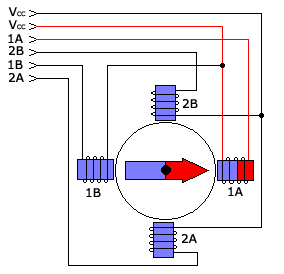
\includegraphics[height=15em]{./img/motor_stepper_unipolar.png}}
					\subcaptionbox{Motorgetriebe\protect\footnotemark\label{fig:Getriebe}}
						{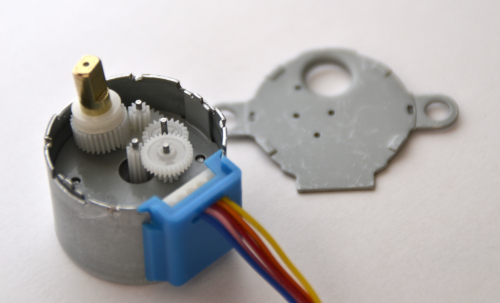
\includegraphics[height=15em]{./img/gear.png}}
					\caption{ Aufbau eines unipolaren Schrittmotors.
					\label{fig:imgMotor}}
				\end{figure}
				\footnotetext{\textcopyright Alexander Hinkel [Quelle:\cite{Schrittmotor_Getriebe}]}
		\newpage
		\section{Realisierung der Schaltung}
			\subsection{Motorsteuerung}
			\label{sec:Motorsteuerung}
				%ULN, Darlington, Motormesswerte der Wiederstände, Berechnung der Ströme und Leistungen
				Eine Darlington-Schaltung ist eine Schaltung zweier Transistoren mit hoher Stromverstärkung und wird zur Schaltung beziehungsweise Steuerung größerer Lasten eingesetzt [Böhmer et al. \cite[S.290]{Darlington}]. Dabei können die nötigen Steuerströme gering gehalten werden. 
				\newline Der hier verwendete ULN2003 beinhaltet mehrere Darlington-Transistoren in einem Gehäuse und verstärkt die Steuersignale des Arduinos ohne dessen Ausgänge mit zu hohen Stromstärken zu belasten. Gemäß Datenblatt ist die Kollektor-Emitter-Sättigungs-Spannung im leitenden Zustand zwischen 1,1 und 1,3 Volt bei oben angenommener Stromstärke im Einphasenbetrieb und 1,3 bis 1,6 Volt bei Zweiphasenbetrieb des Motors (Gleichung \ref{eq:StromMinMax}). Bei der höchsten angenommenen Sättigungsspannung von 1,6 V ergibt sich ein Potenzialunterschied an den jeweiligen Wicklungen von 3,4 V.
				Die Messung der Widerstände der einzelnen Halbspulen\footnote{Messung durch Multimeter: \textit{testo67-2}} des verwendeten Motors ergibt, dass jede Phase etwa 23 $\Omega$ Widerstand hat. Bei Vollschrittbetrieb des Motors, bei dem je genau eine Phase geschaltet wird, lassen sich die Ströme daher berechnen:
				\begin{equation}
					I_{Phase}=\frac{\text{Versorgungsspannung (5V)} - \text{Sättigungsspannung}}{\text{Phasenwiderstand (23$\Omega$)}}
				\end{equation}


				\vspace{3em}
				Berechnung der maximalen und minimalen Stromstärke:
				\begin{equation}
					I_{max}=\frac{3.4 V}{11.5 \Omega}=295.6 mA \hspace{10em}
					I_{min}=\frac{3.7 V}{23 \Omega}=160.8 mA
				\end{equation}
				\newline
				Die berechneten Stromstärken liegen deutlich unter dem Maximalwert des ULN2003, daher kann eine beliebige Variante der Motorsteuerung gewählt werden, ohne diesen zu beschädigen (siehe Anhang \ref{sec:data}). 
				\begin{figure}[htbp]
					\centering
					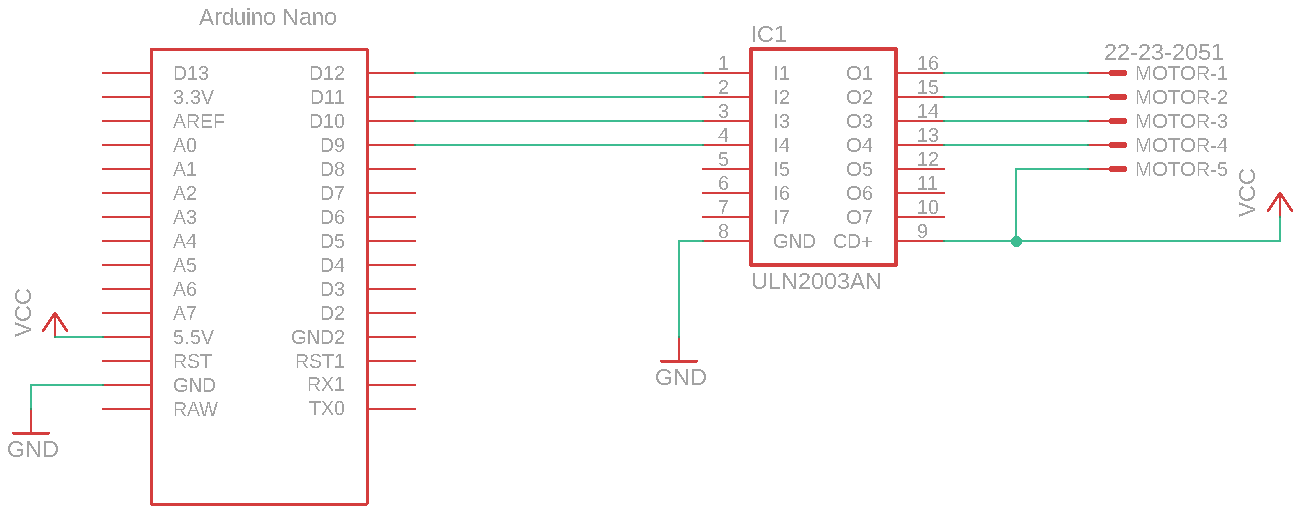
\includegraphics[width=\linewidth]{./img/Motorsteuerung.png}
					\caption{ Ansteuerung des Motors durch Arduino und  Darlington-Transistortreiber ULN2003.
					\label{fig:imgMotorsteuerung}}
				\end{figure}
			\newpage
			\subsection{IR-Empfänger}
			\label{sec:IR}
				%FilterKondensator, FrqBank, Pullup
				Das verwendete Infrarotempfänger-Modul TSOP4838 beinhaltet einen Fotosensor, Demodulator und Vorverstärker. Signalimpulse mit einer Trägerfrequenz von 38 kHz werden Empfangen, demoduliert, vorverstärkt und an den Output gegeben. Durch den Pull-up-Widerstand wird dieses Signal weiter verstärkt und an den Arduino Nano geleitet. Der analoge Eingang A5 des Arduinos kann als digitaler Eingang betrieben werden und wird hier benutzt, um das Platinenlayout übersichtlich zu halten. Zur Filterung von Störsignalen dient der RC-Tiefpassfilter.

				Tastendrücke auf einer Fernbedienung in diesem Frequenzbereich werden vom Empfänger als Hexadezimalcode weitergegeben. Bei Betrieb des Arduinos und zeitgleich verbundener serieller Schnittstelle, können die demodulierten Hexadezimalcodes über den seriellen Monitor der Arduino IDE ausgegeben werden.

				\hspace{5em}
				\begin{figure}[htbp]
					\centering
					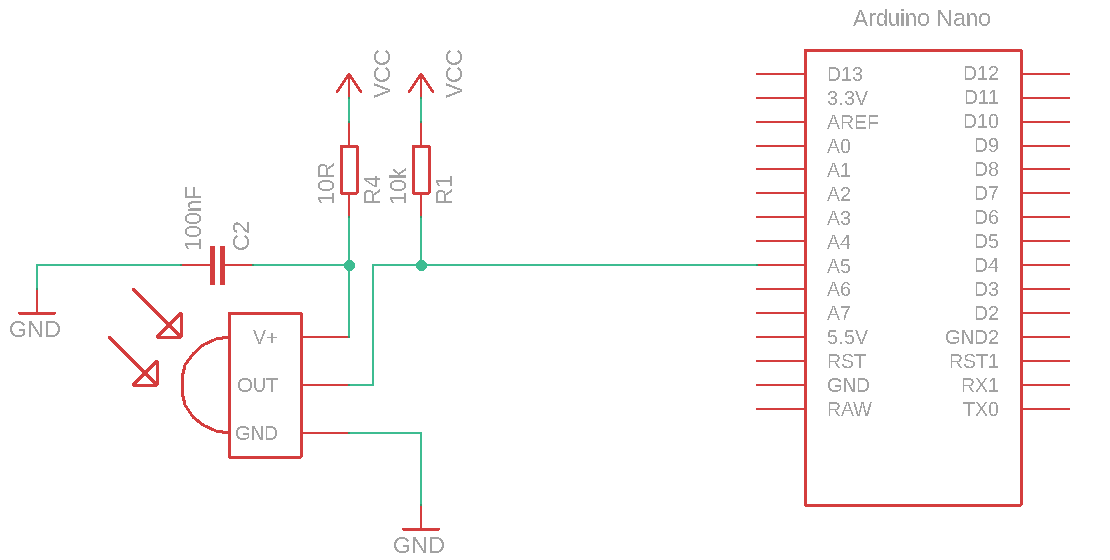
\includegraphics[width=\linewidth]{./img/ir.png}
					\caption{ Infrarot-Empfänger mit Pull-up-Widerstand und Filter.
					\label{fig:imgIR}}
				\end{figure}
			\newpage	
			\subsection{Display}
			\label{sec:Display}
				%LCD 16.2, Pinbelegung, Kontrastberechnungl
				Das im RotaCon verwendete LCD-Display ist ein \textit{TC1602B-01}. Wie in Kapitel \ref{sec:Theorie Hardware} erläutert, besteht der RotaCon aus 2 Gehäusen. Neben dem IR-Empfänger befindet sich auch das Display in einem für den Nutzer sichtbaren Gehäuse, dass mit einem D-Sub-Kabel\footnote{D-Sub ist eine Bauform für Steckersysteme mit n Datenpolen und einer zusätzlichen Masse. Im RotaCon wird ein 9 Pol D-Sub benutzt.} verbunden ist. Die meisten Pins sind direkt mit dem Arduino Nano verbunden, werden rein über Software gesteuert und sind in \ref{sec:Gesamtschaltung} beschrieben oder dem Datenblatt zu entnehmen. Display-Pin 3 setzt zusätzlich einen Spannungsteiler voraus, um den Bildschirmkontrast festzulegen. Die dafür im RotaCon benutzten Widerstandsgrößen sind durch den Einsatz eines Potentiometers ($10k\Omega$) ermittelt und ergeben die optimale Lesbarkeit bei einer Versorgungsspannung des verwendeten Displays von 5V.
				\begin{figure}[htbp]
					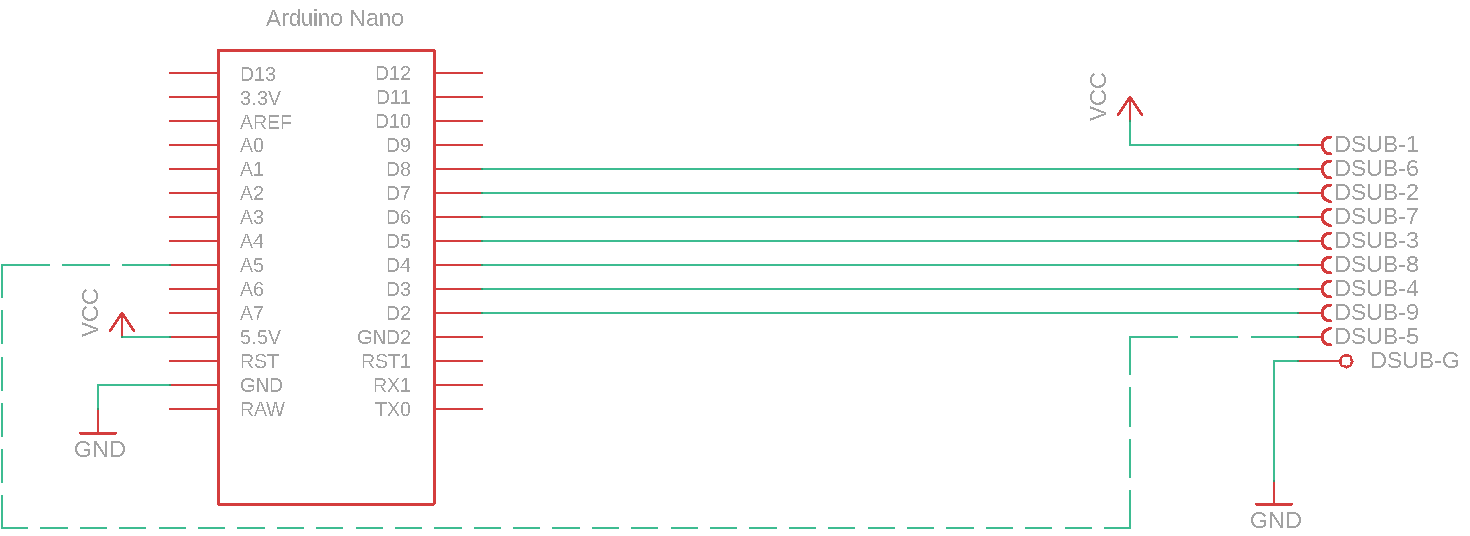
\includegraphics[width=\linewidth]{./img/dsub2.png}
					\label{fig:imgDisplay}
				\end{figure}
				\begin{figure}[htbp]
					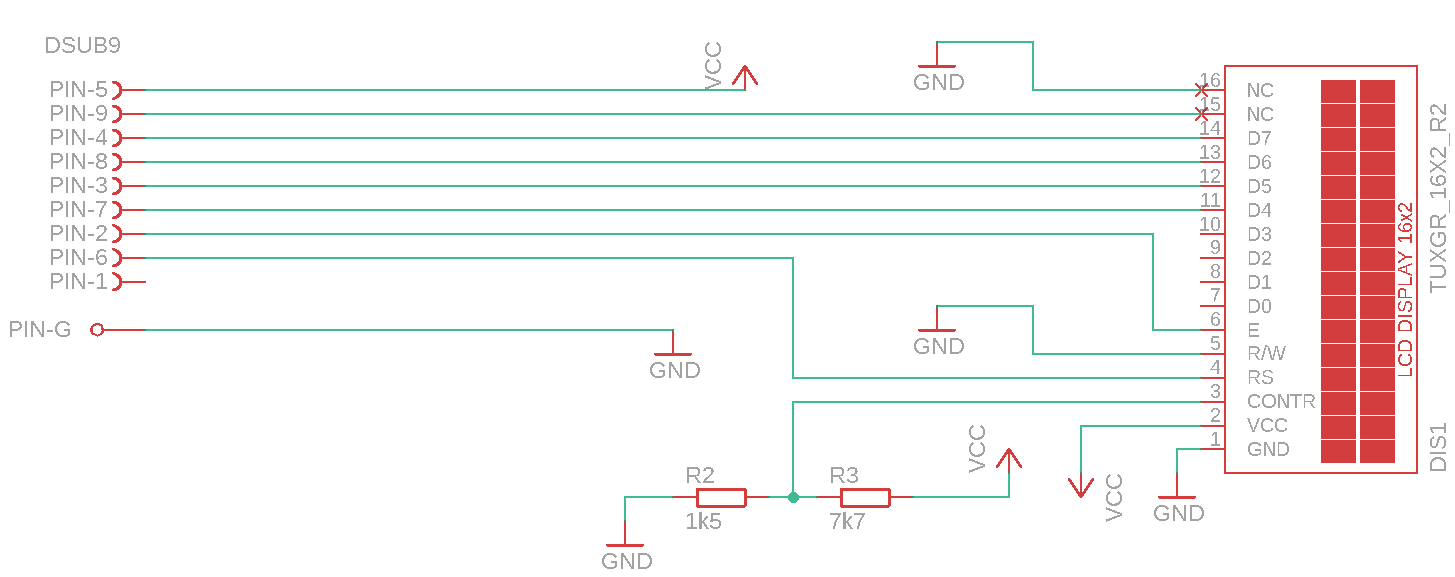
\includegraphics[width=\linewidth]{./img/display2.png}
					\caption[D-Sub-Pinbelegung für Display und IR-Receiver]{D-Sub-Pinbelegung für Display und IR-Receiver(gestrichelte Linie).
					\label{fig:imgDSUB}}
				\end{figure}

				An dieser Stelle sei genannt, dass durch die Spiegelung der D-Sub-Schnittstelle die Pin-Nummern beachtet werden müssen. So ist beispielsweise die Versorgungsspannung bei dem D-Sub der Hauptplatine auf Pin 1, bei der Display-Platine jedoch auf Pin 5. (siehe Abbildung \ref{fig:imgDSUB})
			\newpage
			\subsection{Anschlagerkennung durch Strommessung}
			\label{sec:op}
				%OP-Verstärker, Berechnung, vergleich mit Messungen/Erwartungen (TABELLE?)
				 Durch eine zusätzliche Schaltung wird der durch den Motor verbrauchte Strom gemessen. Dadurch wird untersucht, ob der Motor bei Erreichen der Maximalstellung des Potentiometers vom Normalstromverbrauch abweicht und dies softwaretechnisch zur Motorsteuerung beitragen kann. Durch einen nicht invertierenden Verstärker wird der Strom zu einer für den Arduino auswertbaren Spannung gewandelt. Die allgemeine Funktionsweise von Operationsverstärkern wird hier nicht tiefer erläutert. 
				 \newline Aufgrund der in Abschnitt \ref{sec:Motorsteuerung} genannten Sättigung wird die Ausgangsspannung (U$_{a}$) der Operationsverstärkerschaltung als Ausgangsgröße auf 4V festgelegt. Diese soll durch den in den Arduino integrierten Analog-Digitalwandler ausgewertet werden können. Für einen möglichst geringen Leistungsverlust, werden 2 parallel geschaltete Strommess-Widerstände (R1 und R2 in Abb.\ref{fig:imgOP}) eingesetzt und die Eingangsspannung (U$_{e}$) auf 0,5V festgelegt. R3 und R4 in der Schaltung haben einen Widerstand von 4,7 $k\Omega$. Durch die angenommenen Spannungen ergibt sich ein benötigter Verstärkungsfaktor (V) von 8, welcher wiederum zur Berechnung von R5 ausschlaggebend ist (siehe Gleichung \ref{eq:op}).
				\vspace*{1.5em}
				\begin{equation}
					\label{eq:op}
					V = \frac{U_a}{U_e} =\frac{4V}{0,5V}= 8 \hspace{6em} V = 1+\frac{R5}{R4} \hspace{6em} R5 = R4\cdot(V-1) = 32900\Omega \equiv 33k\Omega
				\end{equation}

				\begin{figure}[htbp]
					\centering
					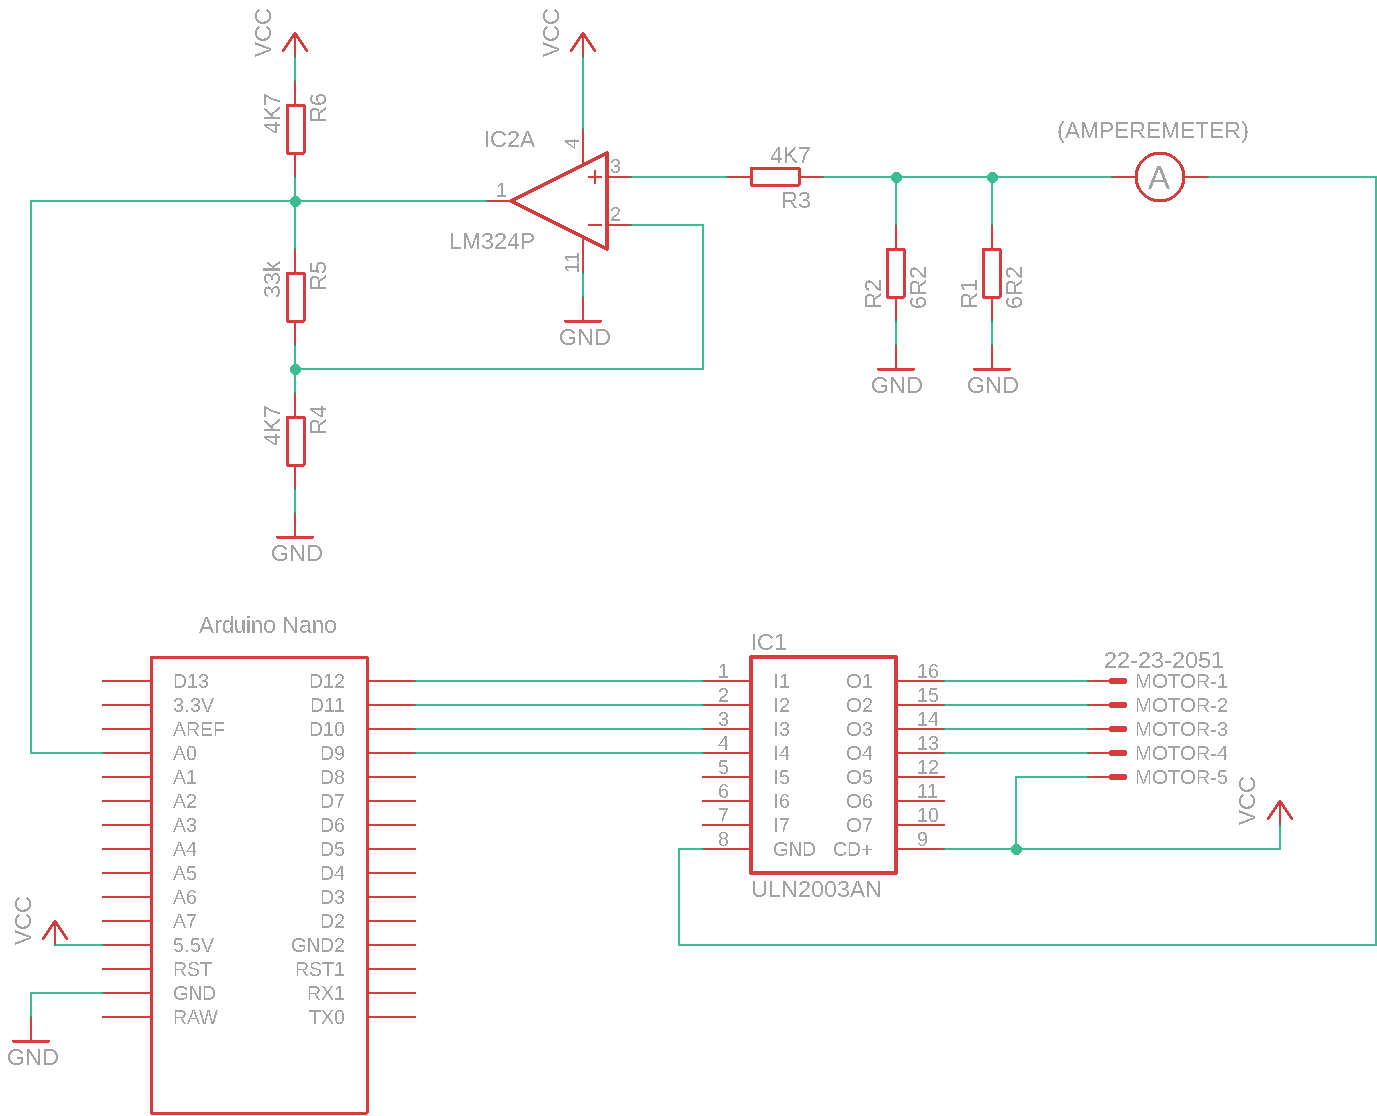
\includegraphics[width=\linewidth]{./img/op2.png}
					\caption[Einsatz eines nicht-invertierenden Verstärkers zur Strommessung]{Einsatz eines nicht-invertierenden Verstärkers zur Strommessung (LM324N)
					\label{fig:imgOP}}			
				\end{figure}
				\newpage

				Der in Abschnitt \ref{sec:Motorsteuerung} ermittelte Strom wird für diese Berechnung auf 160 mA festgelegt und teilt sich hälftig auf die beiden Messwiderstände R1 und R2 auf an denen je die Eingangsspannung $U_{e}$ anliegt. Durch das ohmsche Gesetz leiten sich daher die Widerstandsgrößen her.

				\begin{equation}
					U_{e}=R1\cdot\frac{I}{2}=0,5V \hspace{6em} R1=R2=\frac{2\cdot U_{e}}{I}=\frac{1V}{0,16A}=6,25\Omega \equiv 6R2
				\end{equation}

				Bei Schaltung einer Phase des Motors misst der Arduino mit dem integrierten A/D-Wandler 3,5V. Durch die bekannte Verstärkung\footnote{Die in dieser Rechnung verwendete Verstärkung ist 7,94 und bezieht sich auf die gemessenen Werte der verbauten Widerstände.} errechnet sich so ein $U_{e}$ von 0,441V am Widerstand R1. Daraus ergibt sich eine errechnete Stromstärke von 145 mA. Das Amperemeter\footnote{Verwendetes Multimeter: testo 760-2} gemäß Abb. \ref{fig:imgOP} misst 144mA. Somit entsprechen die im seriellen Monitor der Arduino IDE gelisteten Werte, den etwa tatsächlichen Werten der Schaltung und können ausgewertet werden. Der verwendete Widerstand 6R2 hat einen gemessenen Wert von 6.1$\Omega$.

				\begin{equation}
					\label{eq:ue}
					U_{e}=\frac{U_{a}}{\text{V}} = \frac{3.5V}{7.94} = 0.441V \hspace{6em} I=\frac{2\cdot U_{e}}{R1}=\frac{2\cdot 0.441V}{6.1\Omega}=0.145A
				\end{equation}

				Induktivitäten benötigen eine gewisse Zeit, um sich zu laden bzw. entladen und ein Schritt des RotaCons entspricht 64 Schaltvorgängen, die mit einer Frequenz von 500Hz (siehe Abschnitt \ref{sec:Software}) stattfinden. Somit wird jede Phase einmal alle 8ms geschaltet wobei 2 Phasen zu je einer Induktivität gehören. Der Strom ist daher nicht konstant und der Zeitpunkt des Messens müsste möglichst am Ende eines Schaltimpulses liegen.
				
				\vspace{1.5em}
				\begin{figure}[htbp]
					\label{fig:spule}
					\centering
					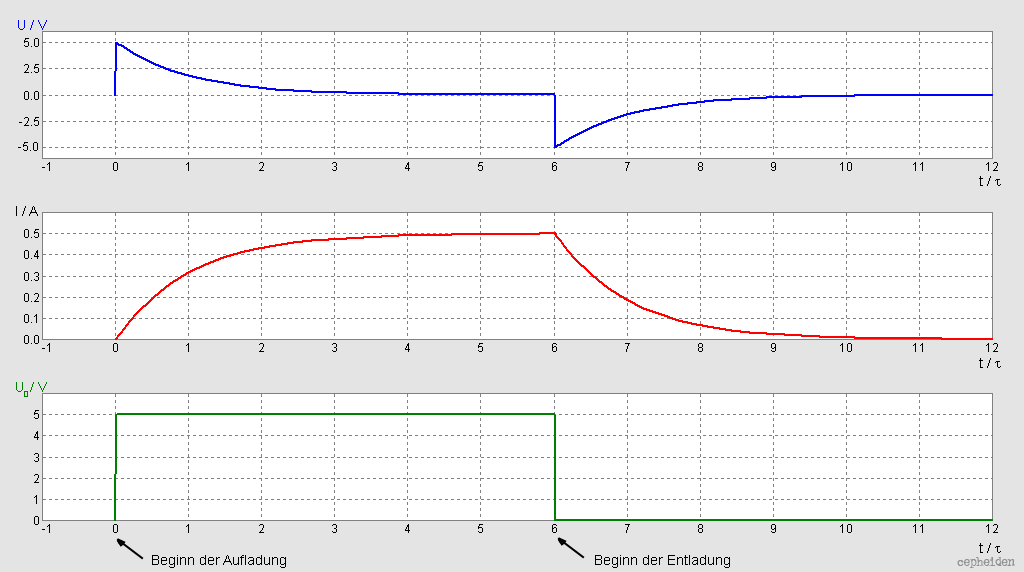
\includegraphics[width=0.7\linewidth]{img/Spule.png}
					\caption[Auf- und Entladung einer Spule]{Auf- und Entladung einer Spule [Bildquelle: \cite{Spule}]}
				\end{figure}	
				
				Die Messung im RotaCon ist jedoch unmittelbar nach dem Schaltbeginn um möglichst große Differenzen bei Erreichen des Potentiometer-Anschlags zu erkennen.
				\newline Ist der Anker des Schrittmotors blockiert, während die Phasen weiterhin geschaltet werden, so ändert sich das Verhältnis der Magnetfelder und ein zusätzlicher Strom wird induziert. Daher ist die Differenz zwischen Minimalwert und Maximalwert der Ströme beim Erreichen des Anschlags geringer. Der Anschlag ist somit zwar erkennbar,
				aber diese Differenz ist nicht konstant. Die kleinste gemessene Differenz $\Delta U_{a}$ beträgt 0,3V und entspricht etwa einem $\Delta U_{e}$ von 0,04V und somit etwa 13mA. Minimale Schwankungen werden mit verstärkt tragen somit bereits zur Ungenauigkeit bei (Berechnung gem. Gleichung \ref{eq:ue}).
			\newpage
			\subsection{Anschlagerkennung durch Endschalter}
				%Redundanz, pullUp
				Redundant zur Strommessung und Auswertung besitzt der RotaCon zwei Endschalter, diese sind Mikroschalter mit Flachhebel und im ''normaly open'' -Modus betrieben. Bei dem Prototypen sind diese Schalter durch Klebemasse befestigt und können je nach Potentiometer beliebig auf dem RotaCon-Gehäuse befestigt werden. Motorachse und Potentiometer sind durch eine flexible Wellenkupplung verbunden. An dieser Kupplung ist zusätzlich eine 25mm Schraube mit M4-Gewinde eingeschraubt, die als Hebel zum Auslösen der Schalter dient. Sobald einer der Schalter ausgelöst wird, wechselt der entsprechende Pin des Arduinos auf LOW und der Motor wird durch Software für diese Drehrichtung gestoppt.
			\subsection{Pinbelegungen}
			\label{sec:Gesamtschaltung}
				%SChaltpläne eventuell als Beginn des Kapitels?
				%Verbindung der Gehäuse mit DSUB9, Polbelegung DSUB
				Durch die Verwendung zweier Platinen und resultierender Kabelverbindung, sind einzelne Signalpfade nur schwer nachzuvollziehen. Folgende Tabelle bietet eine Übersicht aller Pins. Die Platinen sind abgekürzt mit DB(Display-Board) und MB (Motor-Board).
				\begin{table}[htbp]
					\centering
					\caption[Pin-Belegungen]{Pin-Belegungen}
					\label{tab:tabDisplay}
					\begin{tabular}{llllllll}
					\toprule
						\textbf{Arduino} & \textbf{DSUB MB} 	  & \textbf{DSUB DB} 	& \textbf{Leiste DB} 	& \textbf{Display}	 & \textbf{Symbol}   & \textbf{Level} & \textbf{Beschreibung}\\
					\midrule
						--		&--			&--		& Pin 1		& Pin 1		& VSS/GND	& 0V	& Ground\\
						--		&--			&--		& Pin 2		& Pin 2		& VDD/VCC	& 5V	& DP Versorgungsspannung\\
						--		&--			&--		& Pin 3		& Pin 3		& V0/CONTR	& --	& LCD-Kontrast\\
						D2		& Pin 9		& Pin 6	& Pin 4		& Pin 4		& RS		& H/L	& H: Datensignal, L: Befehl\\
						--		&--			&--		& Pin 5		& Pin 5		& R/W		& H/L	& H: Lesen, L: Schreiben\\
						D3		& Pin 4		& Pin 2	& Pin 6		& Pin 6		& E			& H/L	& Enable Display\\
						--		&--			&--		& --		& Pin 7-10	& D0-D3		& H/L	& Display-Daten\\
						D4		& Pin 8		& Pin 7	& Pin 7		& Pin 11	& D4		& H/L	& Display-Daten\\
						D5		& Pin 3		& Pin 3	& Pin 8		& Pin 12	& D5		& H/L	& Display-Daten\\
						D6		& Pin 7		& Pin 8	& Pin 9		& Pin 13	& D6		& H/L	& Display-Daten\\
						D7		& Pin 2		& Pin 4	& Pin 10	& Pin 14	& D7		& H/L	& Display-Daten\\
						D8		& Pin 6		& Pin 9	& Pin 11	& Pin 15	& A			& 5V	& LED-Backlight Anode\\
						--		&--			&--		& Pin 12	& Pin 16	& K			& 0V	& LED-Backlight Kathode\\
						D9		&--			&--		& --		& --		& Orange	& H/L	& Motor (Spule 1a)\\
						D10		&--			&--		& --		& --		& Gelb		& H/L	& Motor (Spule 2a)\\
						D11		&--			&--		& --		& --		& Pink		& H/L	& Motor (Spule 1b)\\
						D12		&--			&--		& --		& --		& Blau		& H/L	& Motor (Spule 2b)\\
						A5		& Pin 5		& Pin 1	& --		& --		& --		& H/L	& IR-Receiver\\
						--		& Pin 1		& Pin 5	& --		& --		& VCC		& 5V	& VCC\\
						A0		& --		&--		& --		& --		& --		& 0-5V	& A/D Strommessung Motor\\
						A1		& --		&--		& --		& --		& --		& H/L	& Taster 1\\
						A2		& --		&--		& --		& --		& --		& H/L	& Taster 2\\
	
					\end{tabular}
				\end{table}
				\newpage
			\subsection{Gesamtschaltung der Display-Platine}
				Da das Display durch seine Platzierung im Displaygehäuse von der Platine getrennt ist, wird eine Pinleiste auf der Platine eingesetzt. Display und Platine sind durch Kabelbrücken miteinander verbunden.
				\vspace{3em}
				\begin{figure}[htbp]
					\centering
					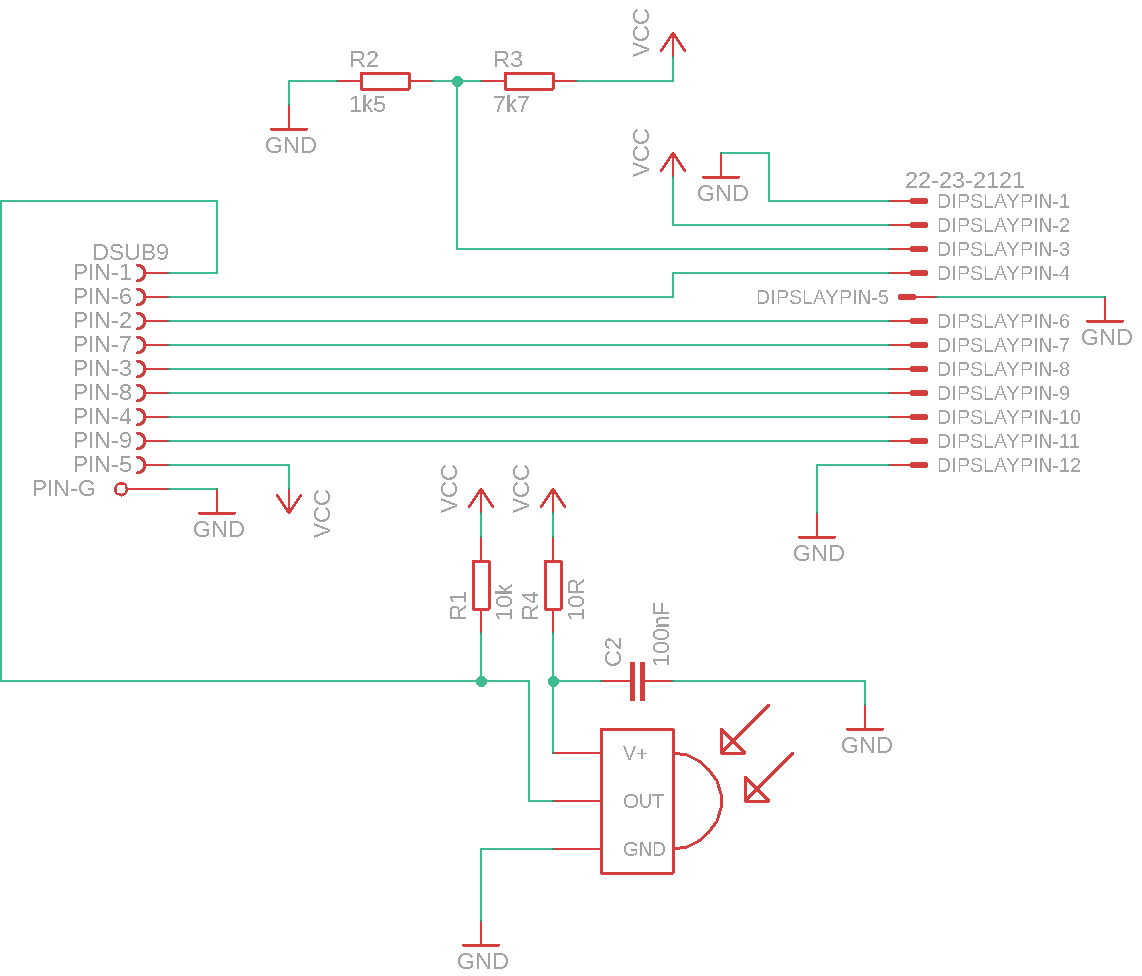
\includegraphics[width=\linewidth]{./img/DisplayComplete.png}
					\caption{Finale Schaltung der Display-Platine.
					\label{fig:imgDPComp}}			
				\end{figure}
				\newpage
			\subsection{Gesamtschaltung der Motor-Platine}
				Die Endschalter sind ebenfalls separat zur Hauptplatine und daher nur als Steckverbindung zu erkennen. Diverse Testpunkte sind in die Schaltung integriert. Die USB-Spannungsquelle sowie zusätzliche Klemmen für eine redundante Spannungsversorgung wurden hinzugefügt. Ein Anschluss für den Betrieb eines weiteren Ports des Arduinos um eventuelle Erweiterungen durchzuführen ist ebenfalls implementiert (Nano-Pin A3).
				\vspace{3em}
				\begin{figure}[htbp]
					\centering
					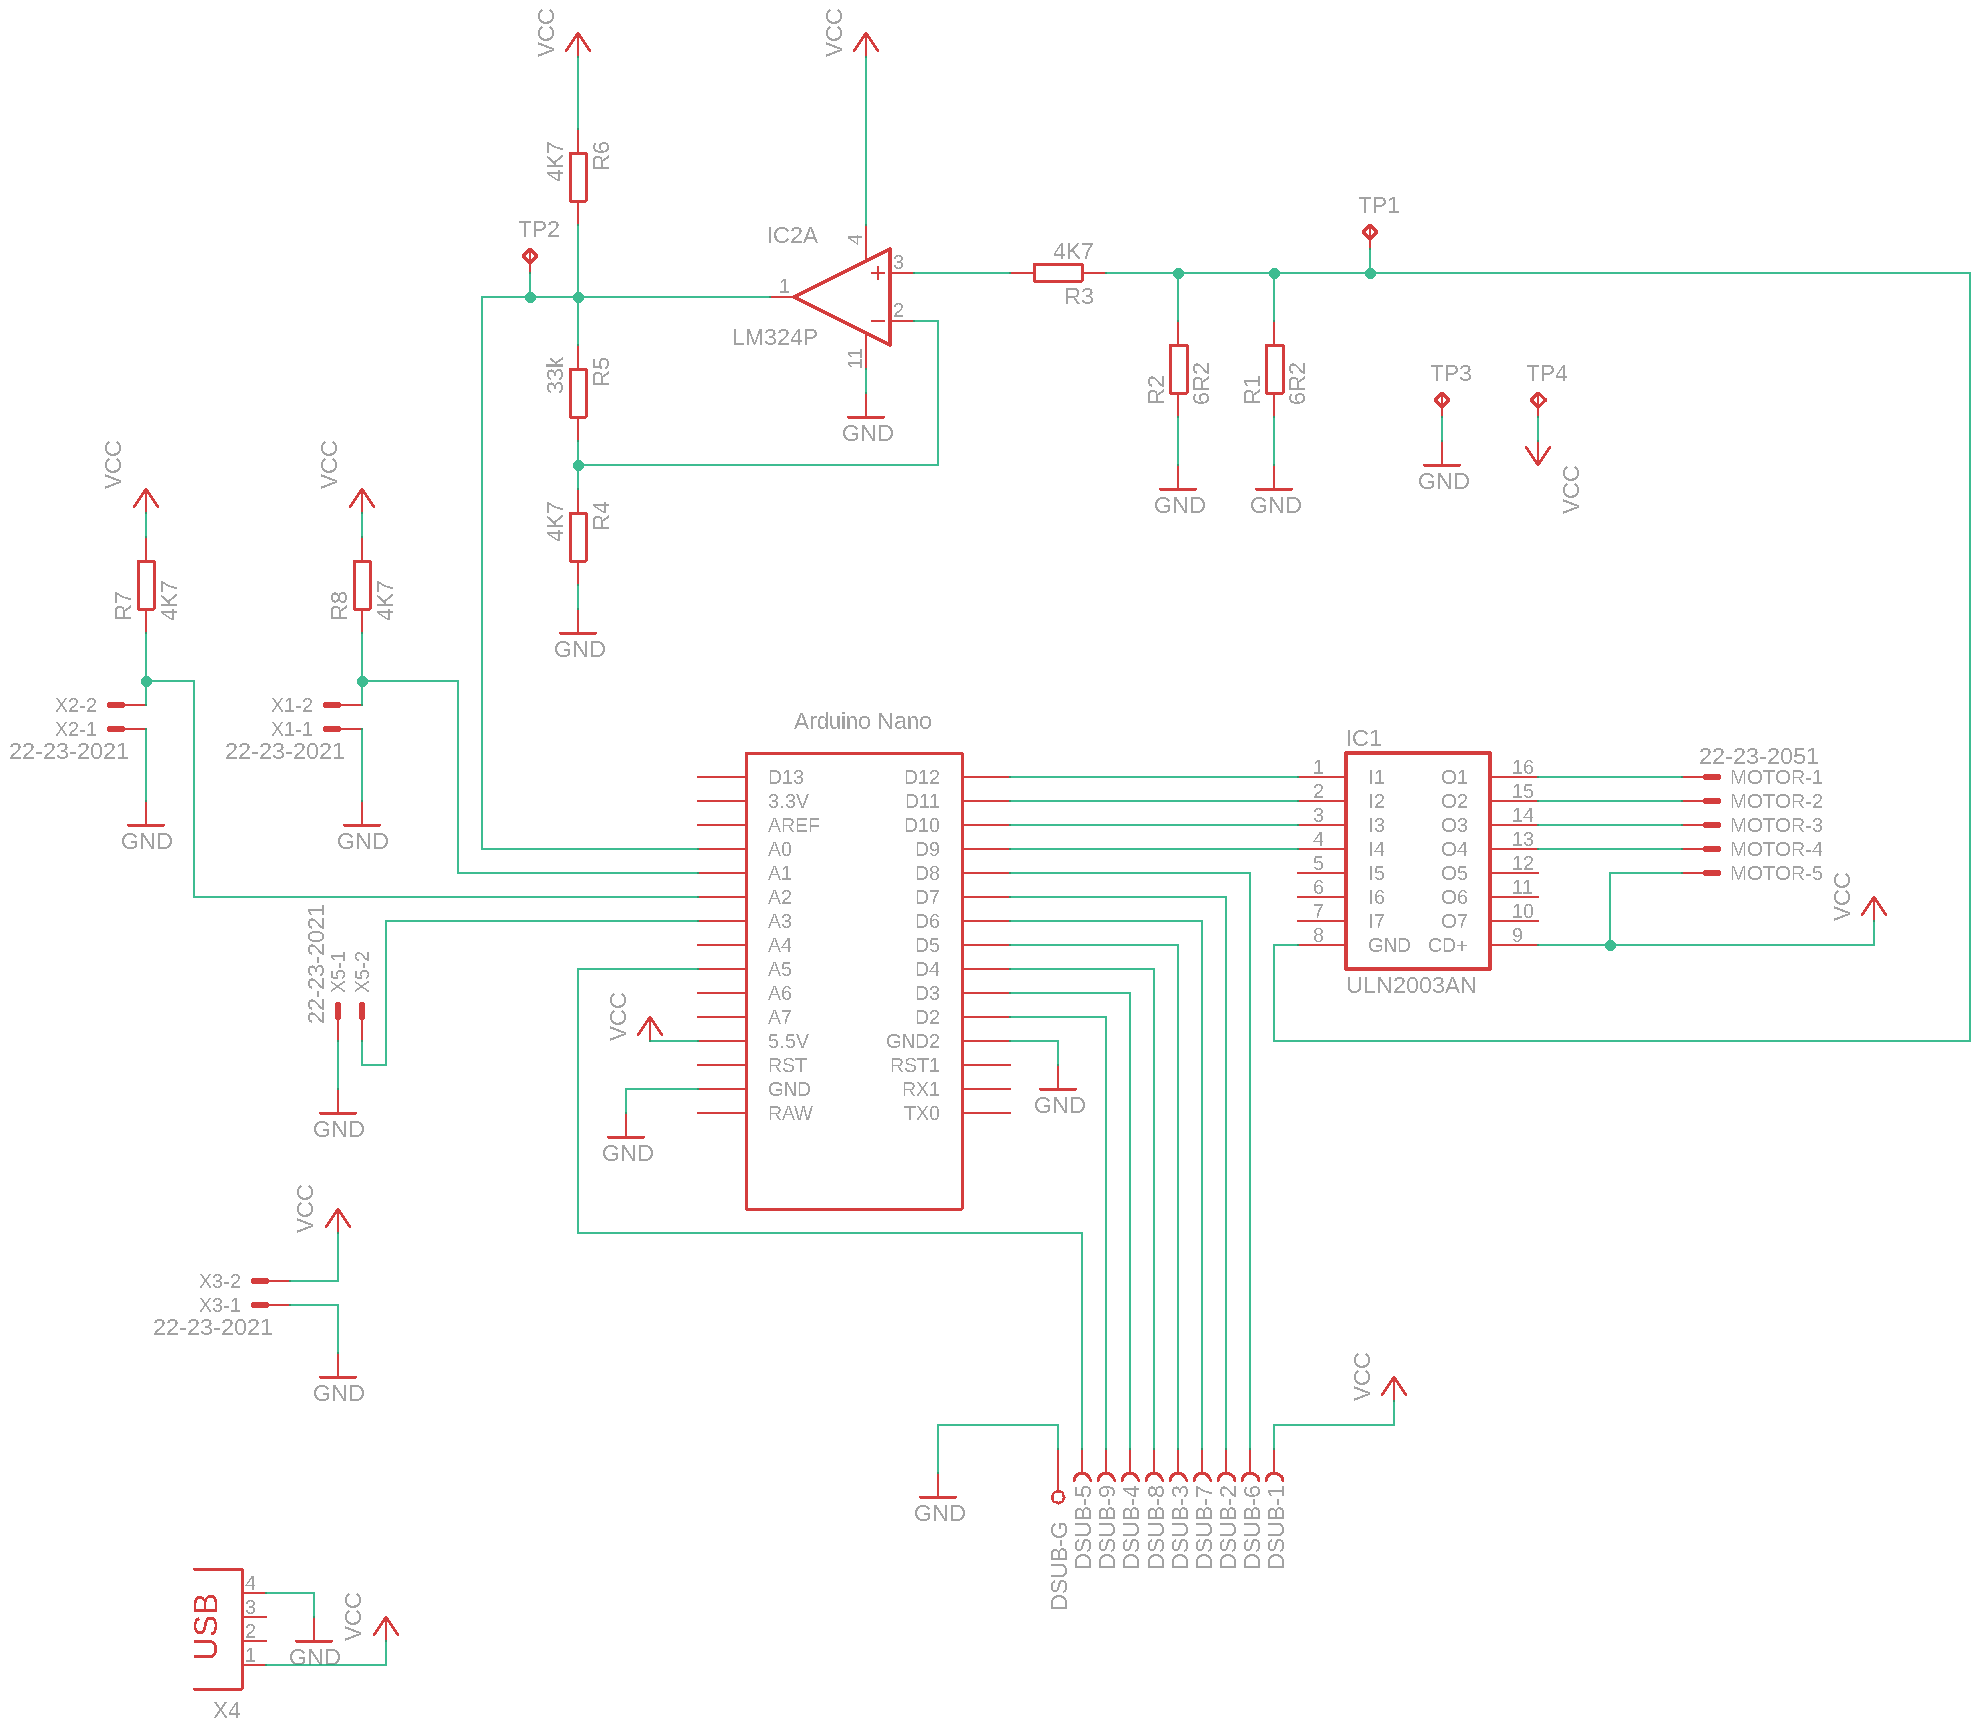
\includegraphics[width=\linewidth]{./img/MotorComplete.png}
					\caption{Finale Schaltung der Motor-Platine.
					\label{fig:MotorComp}}			
				\end{figure}
		\newpage
		\section{Software}
		\label{sec:Software}
			%Matrizen zur Motorsteuerung, case für IR-auslesen, Messung und Minimalwert
			Die Schaltung des Motors ist einfach gehalten. Die vier Phasen-Ports sind über eine Liste angesteuert in der jeweils ein Wert auf HIGH und der Rest auf LOW gesetzt ist. Je nach Rotationsrichtung des Motors muss das HIGH-Bit nun innerhalb der Liste verschoben werden. Da es bei dem Einphasenbetrieb im Vollschrittverfahren nur vier Varianten dieser Liste gibt, wurde hier eine 4x4 Matrix implementiert deren Zeilen je einer dieser Listen entsprechen:

			\begin{lstlisting}[gobble=28, language=C++]
				int stepMatrix[4][4] = {
  				  {HIGH, LOW, LOW, LOW},
  				  {LOW, HIGH, LOW, LOW},
  				  {LOW, LOW, HIGH, LOW},
  				  {LOW, LOW, LOW, HIGH},
				};
			\end{lstlisting}

			Eine volle Umdrehung der Motorachse benötigt 2048 dieser ''Zeilensprünge'' (siehe \ref{sec:Motor}). Als Anhalt für den maximalen Drehwinkel eines Potentiometers wird 320° angenommen. Dies entspricht etwa 1820 Motorschritten. Für die angestrebten 28 bis 30 Lautstärkestufen des RotaCons bedeutet das, dass je 64 Motorschritte für eine Lautstärkestufe passieren müssen. Damit Rotor und Getriebe sich in Bewegung setzen können, ist bewusst ein Delay von 2ms zwischen den einzelnen Schritten implementiert.

			Unmittelbar nach jedem Schritt wird die am A/D-Wandler liegende Spannung abgefragt, die den Motor-Stromverbrauch repräsentiert. Der tiefste Wert nach 64 Schritten wird übergeben und dient zur Feststellung, ob der Motor den Endanschlag des Potentiometers erreicht hat. Sind die Werte oberhalb eines Schwellwertes, ist dies ein Anzeichen, dass der Rotor starr zwischen den schaltenden Elektromagneten steht. Der Schwellwert wurde über Tests im seriellen Monitor ermittelt und liegt bei etwa 2,8V.\newline
			Wird somit ein Anschlag erkannt, oder einer der beiden Taster betätigt, ist die Motorsteuerung für eine Rotation in diese Richtung gesperrt und auf dem Display wird eine Warnung ausgegeben. Das Display lässt sich durch eine Methode deaktivieren, die die Hintergrundbeleuchtung ausschaltet.

			Für die Displaysteuerung und Datenauswertung des Infrarotempfängers werden entsprechende Bibliotheken benutzt. Eine ''Switch-Case-Anweisung'' koordiniert die Eingaben der Fernbedienung. So kann jeder Hexadezimalwert vom IR-Empfänger einer Methode zugewiesen werden. Hält der Benutzer eine beliebige Taste der Fernbedienung gedrückt, so sendet sie den Wert ''0xFFFFFFFF''. Dieser Wert steht für die Wiederholung des zuletzt gesendeten Hex-Codes, daher ist dieser Wert gesondert in der Software betrachtet. (siehe Anhang \ref{sec:Code}) 
			Die aktuelle Motorposition, sowie Lautstärke wird im internen EEPROM-Speicher abgelegt. Sollte der RotaCon vom Strom getrennt werden, bleiben diese Werte somit unverändert.
			
			Die komplette Software ist in dem GitHub-Projekt einsehbar, daher werden weitere Details hier nicht weiter erläutert, um den Umfang dieser Dokumentation übersichtlich zu halten.
		\newpage
		\section{Das Gehäuse}
		\label{sec:Casing}
			Dieser Abschnitt bezieht sich auf Feststellungen aus Kapitel \ref{sec:Design}. Alle Angaben beziehen sich auf die in diesem Projekt verwendeten Materialien. So sind die Maße der Platinen und deren Bohrungen zum Beispiel ausschlaggebend für den Gehäuseentwurf. 
			\subsection{Motorgehäuse}
				Für den Prototypen wurde ein Gehäuse entworfen, das weder verklebt noch vielseitig verschraubt werden muss. Somit kann zu Entwicklungszwecken ein häufiges unkompliziertes Öffnen stattfinden. Exakte Maße sind den detaillierteren technischen Zeichnungen im Anhang zu entnehmen. Ausmaße des Gehäuses ergeben sich durch Platinen- und Motorgröße, da der Motor  komplett im Gehäuse untergebracht ist. Dieses Gehäuse besteht aus zwei einzeln gefertigten Teilen, die mit einem 3D-Drucker produziert werden. 3D-Modell und notwendige Dateien zum Druck sind im GitHub-Projekt abgelegt, variieren jedoch je nach verwendetem Filament und Drucker.
				\vspace{3em}
				%Zeichnung, Modell, gesliced, fertigstück ?
				%Besonderheiten/Probleme
				\begin{figure}[htbp]
					\centering
					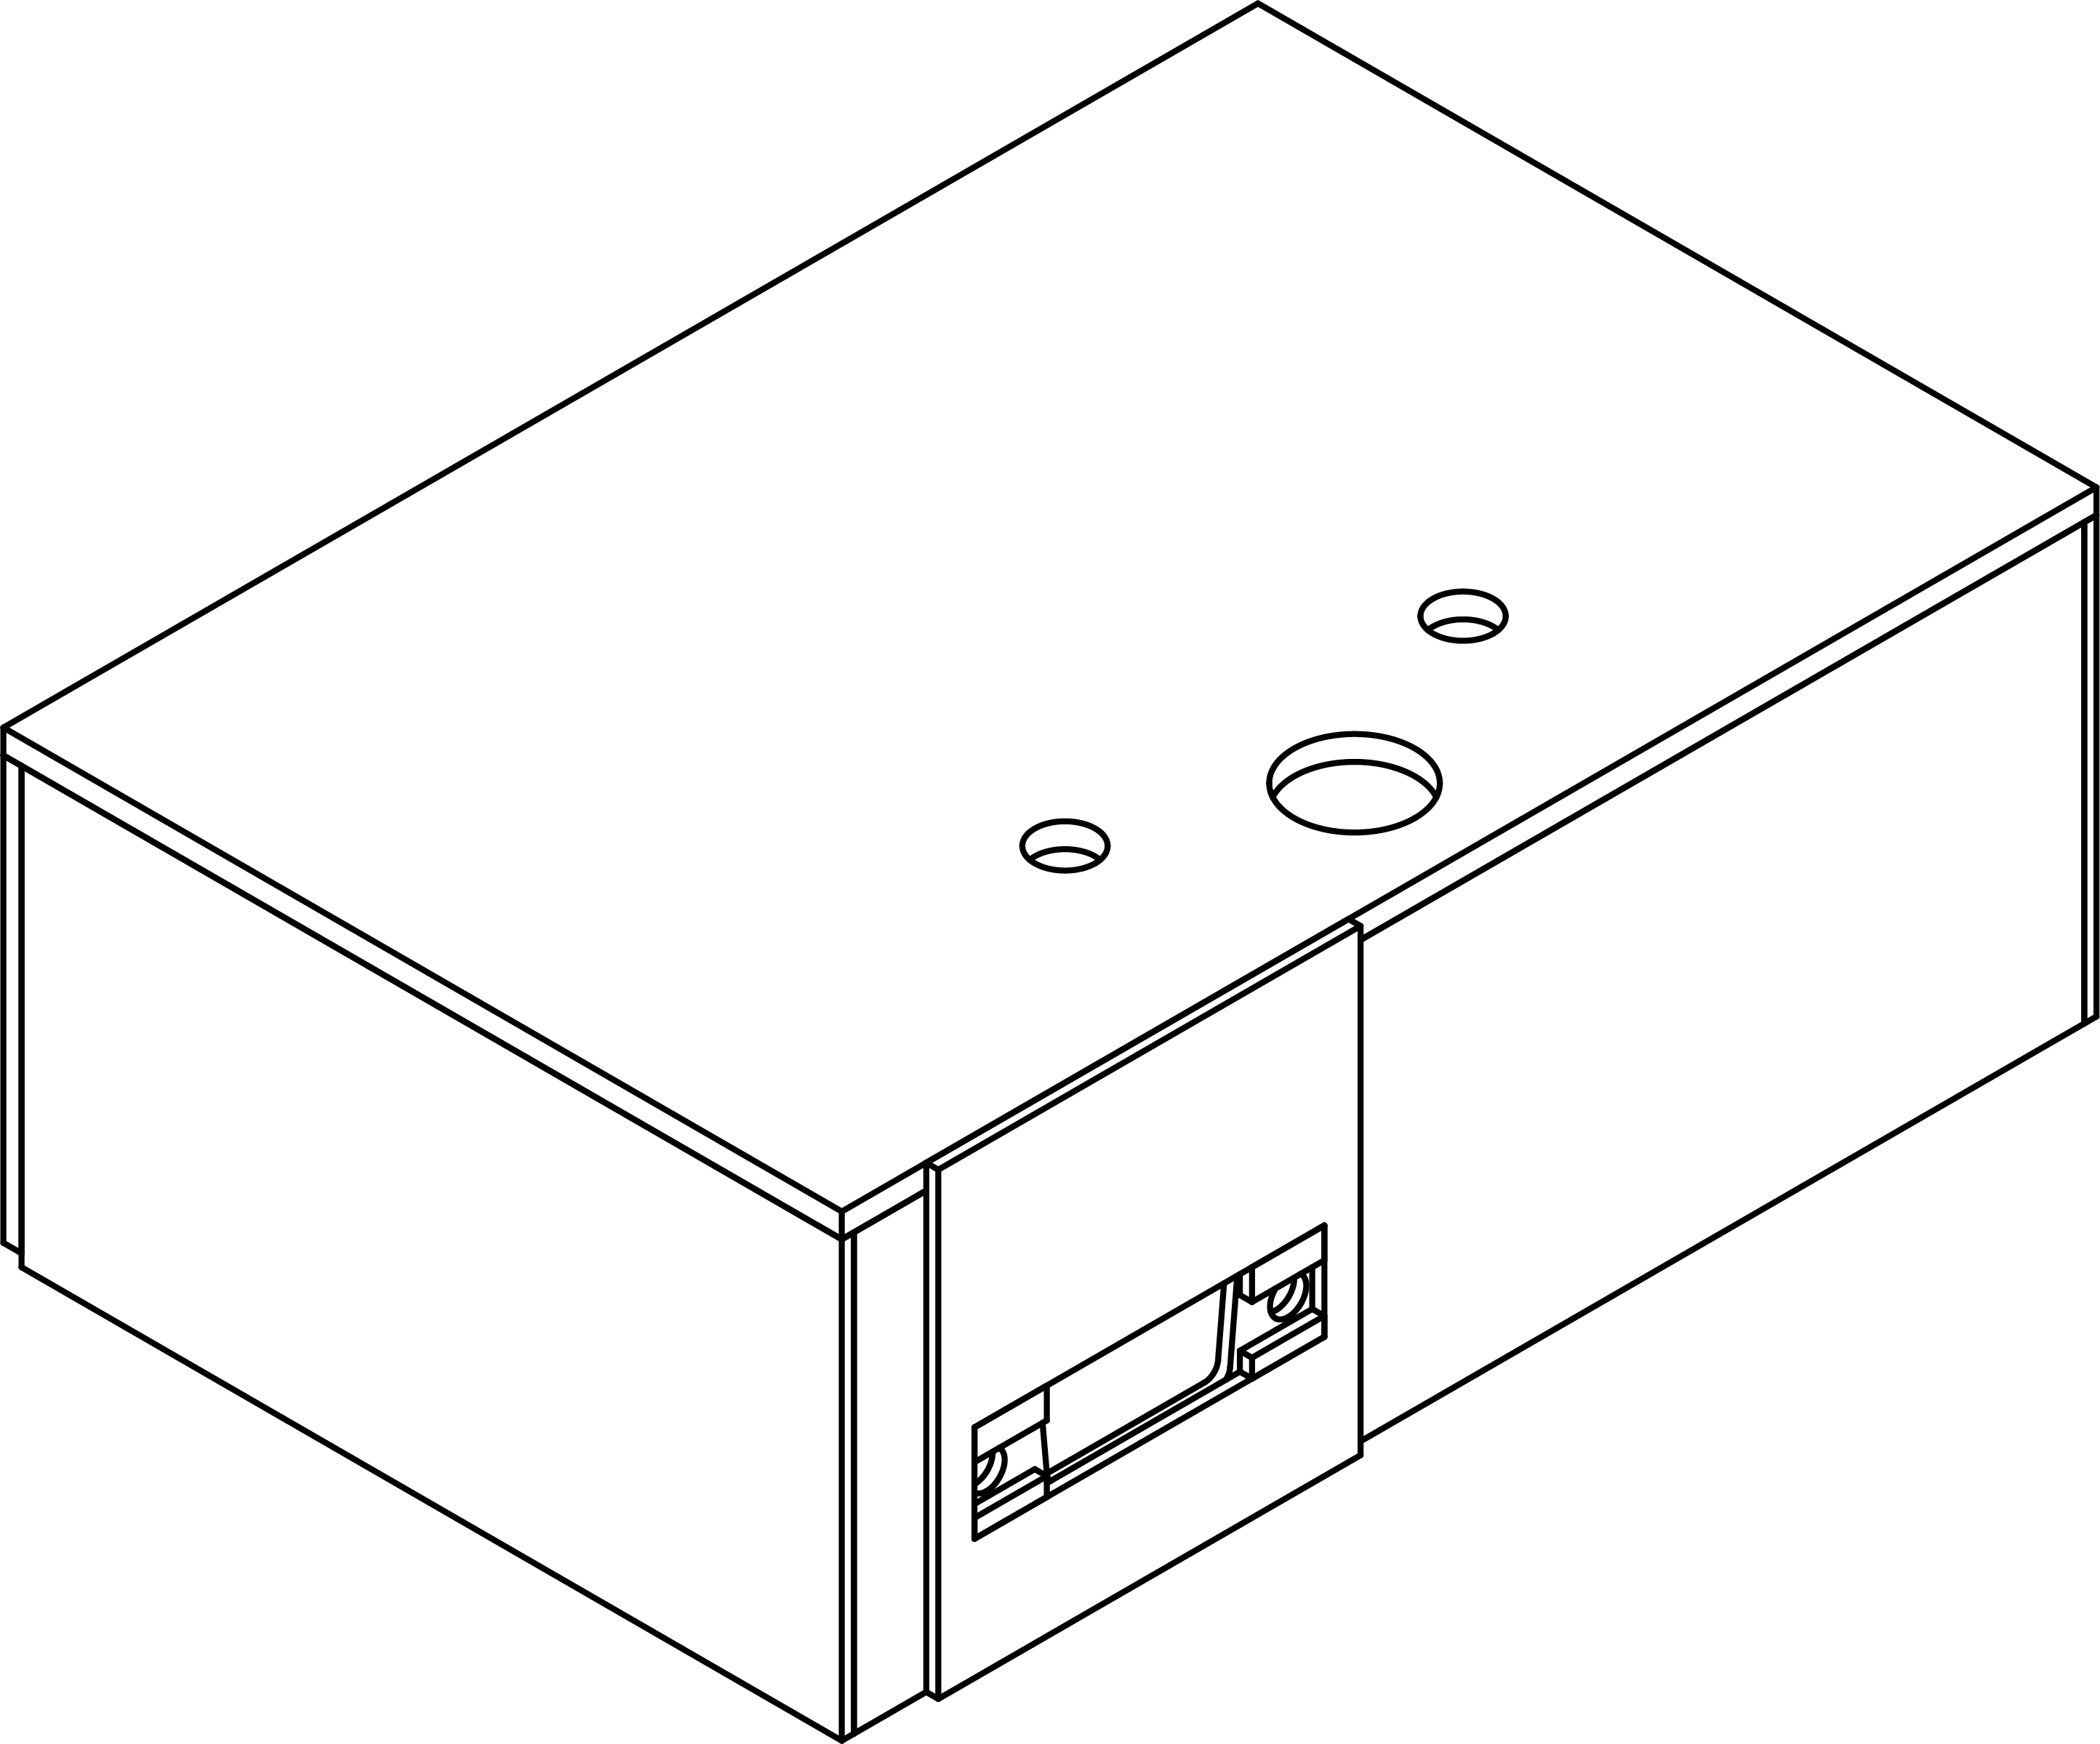
\includegraphics[width=0.75\linewidth]{./img/Motor_Case_Draw.png}
					\caption{Skizze des Motorgehäuses
					\label{fig:imgMotorDraw}}			
				\end{figure}
			\newpage
			\subsection{Displaygehäuse}
				Auch bei diesem Gehäuse wurde darauf geachtet, dass es möglichst einfach geöffnet werden kann. Höhe und Breite sind durch die Displaymaße beeinflusst. Die Öffnung für den IR-Empfänger ist mit möglichst dunkler Folie verdeckt, da Licht der Displaybeleuchtung sonst nach außen scheint. Display und Platine sind in diesem Gehäuse auf Plastikstifte gesteckt und halten ohne Einsatz von Heißkleber oder Schrauben. Durch das 40cm lange D-Sub-Kabel kann dieses Gehäuse frei auf der Oberseite des Lautsprechers platziert werden. Zum einen verbinden keilförmige Haken als Klemmverschluss die beiden Gehäuseteile miteinander, zum anderen sorgt die D-Sub-Steckverbindung für den Zusammenhalt.
				\vspace{3em}
				\begin{figure}[htbp]
					\centering
					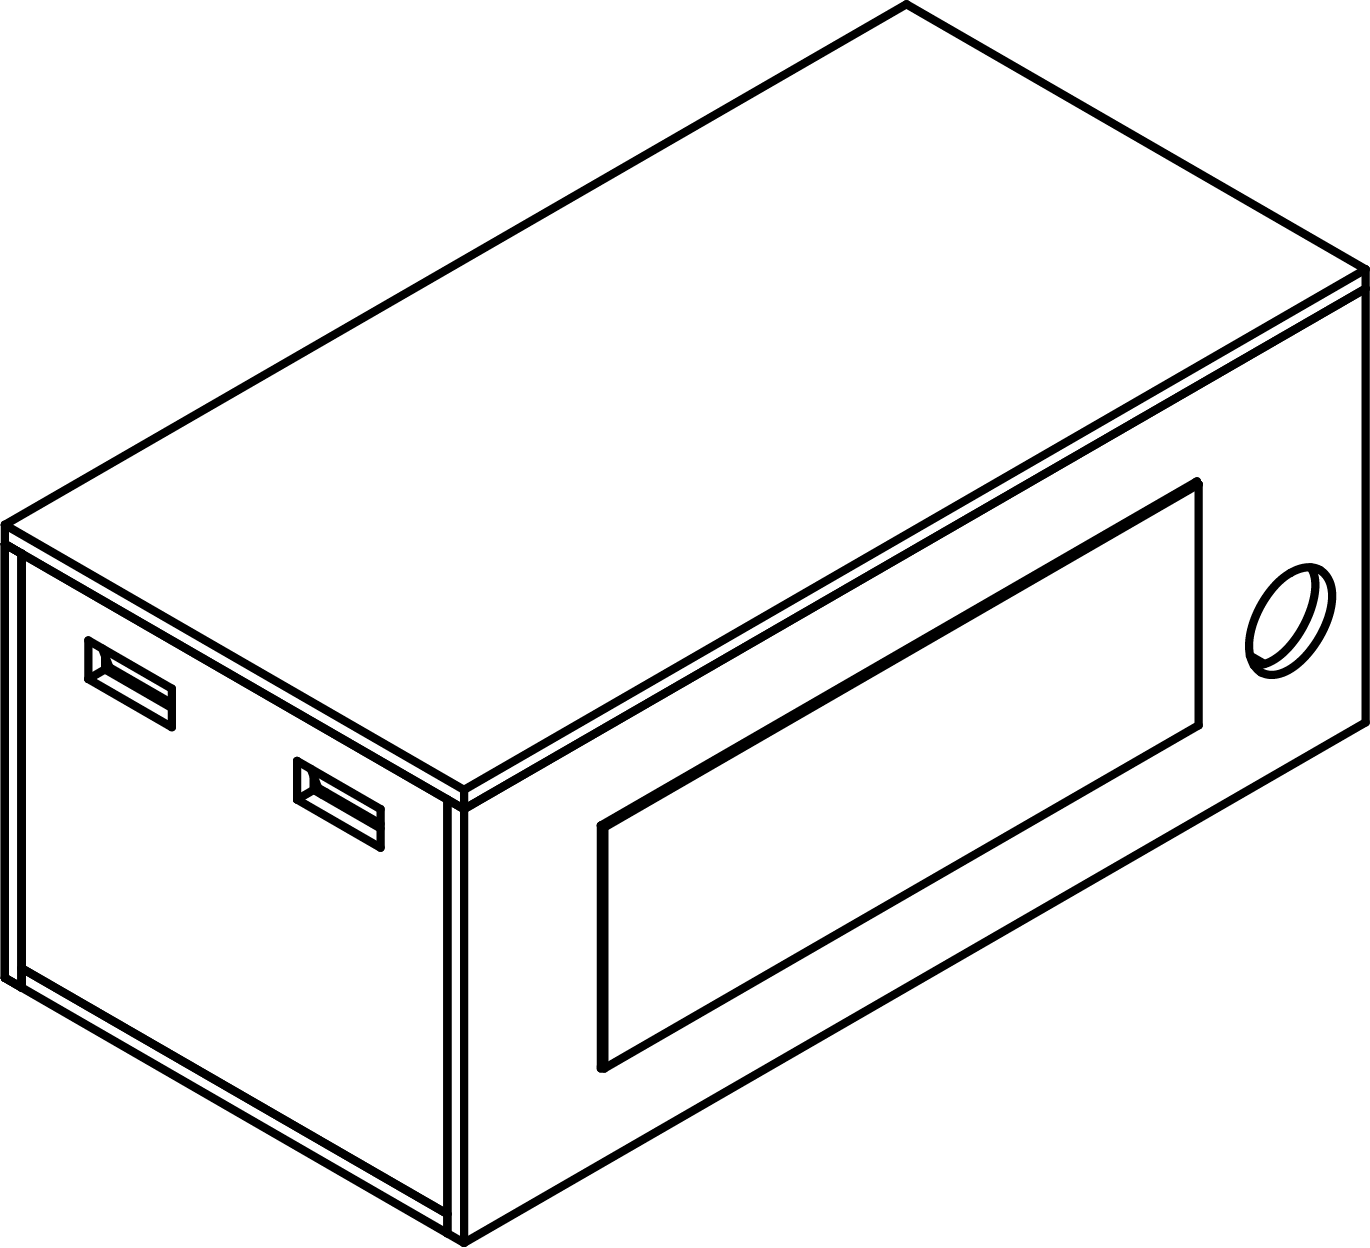
\includegraphics[width=0.75\linewidth]{./img/Display_Case_Draw.png}
					\caption{Skizze des Displaygehäuses
					\label{fig:imgDisplayDraw}}			
				\end{figure}
			\newpage
			\subsection{Gehäuseständer}
				Das Gehäusestativ ist provisorisch und aus entwicklungszeitlichen Gründen nur für den Prototytpen gestaltet. Eine Gewindestange ist in eine Einschraubmutter des lackierten Holzfußes eingeschraubt und durch ein an das Motorgehäuse geklebtes Winkelblech gesteckt. Durch Einsatz zweier Flügelmuttern und Unterlegscheiben lässt sich das Gehäuse somit sehr fein in der Höhe verstellen. Dieses Winkelblech kann bei zukünftigen Versionen zum Beispiel durch Laschen am Motorgehäuse direkt ersetzt werden. Angenehmer für den Benutzer wäre ein Gewinde innerhalb dieser Laschen und die gewindelose Lagerung der Gewindestange im Fuß, so könnte die Gehäusehöhe durch Rotation der Gewindestange eingestellt werden (z.B. via Motor oder Kurbel).
				\vspace{3em}
				\begin{figure}[htbp]
					\centering
					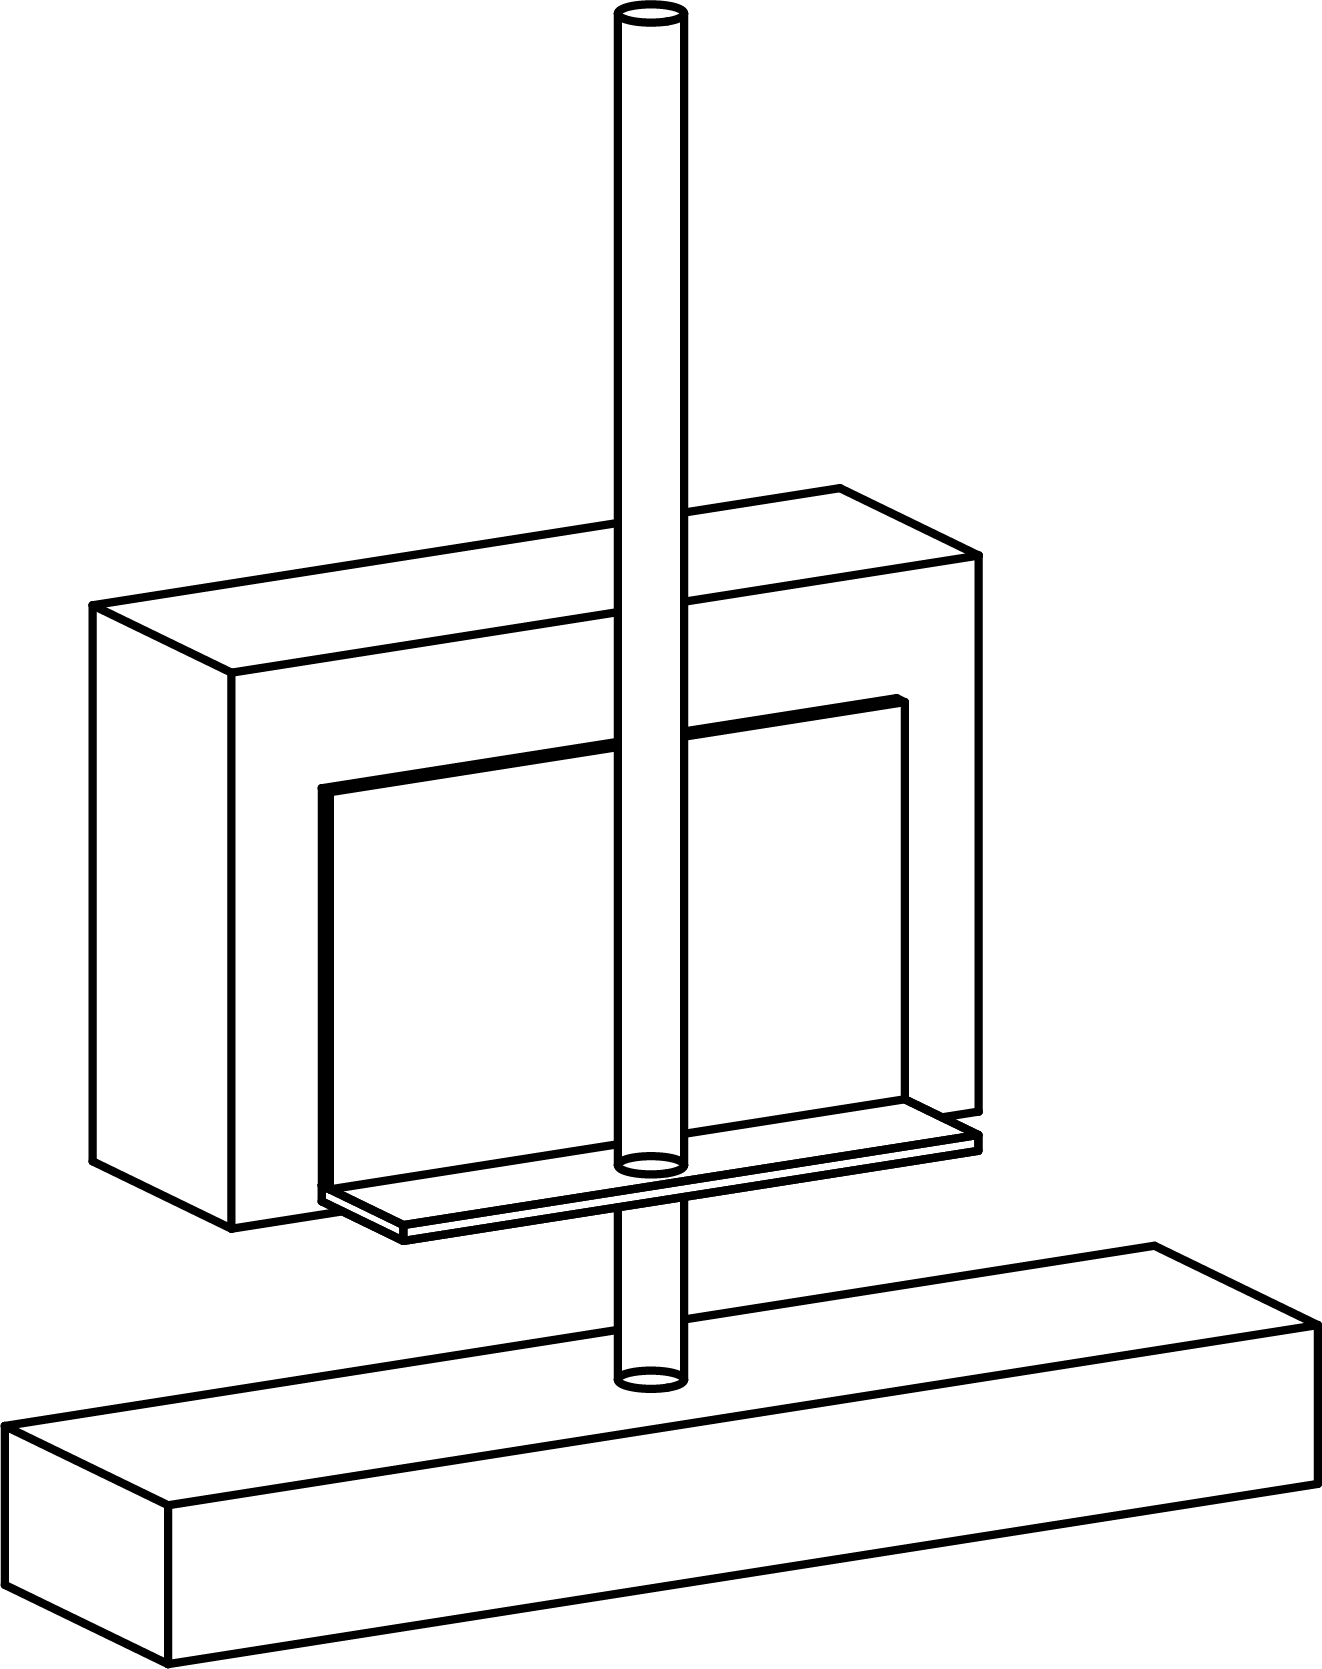
\includegraphics[width=0.75\linewidth]{./img/RotaCon.png}
					\caption{Gehäuseständer des Prototyps
					\label{fig:imgRotaCon}}			
				\end{figure}
		\newpage
	\chapter{Ergebnis}
	\label{sec:Epilog}
		In diesem Kapitel wird die Inbetriebnahme des Prototyps geschildert. Probleme, die bei diesem Projekt aufgetreten sind, werden dargestellt und Lösungsansätze erwähnt. Nach einer kurzen Zusammenfassung des RotaCon-Projekts folgt ein kurzer Abschnitt über mögliche Erweiterungen durch Folgeprojekte.
		\section{Inbetriebnahme}
			\label{sec:HowTo}
			\begin{enumerate}
				\item Abnehmen der Potentiometerkappe am Lautsprecher
				\item Einstellen der Höhe des Motorgehäuses durch Flügelmuttern
				\item Festschrauben der Wellenkupplung (Innensechskant 2mm)
				\item Potentiometer mit Wellenkupplung auf Minimalwert stellen
				\item Anbringen des ersten Tasters durch Klebemasse (Hebel gedrückt)
				\item Stellung auf Maximalwert und letzten Schritt wiederholen
				\item Verbinden beider RotaCon-Gehäuse mit D-Sub-Kabel
				\item Anschließen der Spannungsversorgung
				\item Regeln des Potentiometers per Fernbedienung auf Minimalstellung
				\item Auslösen des Minimalwert-Tasters setzt ''Volume'' auf 0
				\item Der RotaCon ist betriebsbereit
			\end{enumerate}
		\newpage
		\section{Problemdiskussion}
		\label{sec:Probleme}
			\paragraph{Das D-Sub-Verbindungskabel}
			ist sperrig und schränkt die Platzierung des Display-Gehäuses ein. Durch den Einsatz eines $I^{2}C$-Datenbusses können die Pinbelegungen und somit auch die Anzahl der Leitungen im Kabel so reduziert werden, dass ein flexibleres Micro-USB-Kabel verwendet werden kann.
			
			\paragraph{Die Platzierung der Endschalter}
			mit Klebemasse ist unzweckmäßig aber für den ersten Prototyp ausreichend. Eine in das Gehäuse integrierte Ringscheibe, auf der die beiden Endschalter verschoben und befestigt werden können ist eine zweckmäßigere Variante. Darauf wurde jedoch aus Kosten- und Aufwandsgründen bisher verzichtet.
			
			\paragraph{Die Strommessung}
			ist ein guter Ansatz, jedoch noch nicht ausreichend um sichere Aussagen über die Stellung des Potentiometers treffen zu können. Je nach Menge der Eingangssignale von der Fernbedienung oder der Leichtgängigkeit des Potentiometers variieren die gemessenen Werte. Weitere Tests durch Variation des Motorbetriebes (Softwaretechnisch) und damit verbundener Änderung der Messwiderstände können Abhilfe schaffen, wurden aus zeittechnischen Gründen in diesem Projekt jedoch nicht durchgeführt.

		\section{Zusammenfassung}
			Viele aktive Lautsprechersysteme werden über einen am Lautsprechergehäuse befindlichen Potentiometer geregelt. Daher ist es üblich diese Pegel stets auf Maximalwert zu stellen und die tatsächliche Lautstärke über den Signalpegel zum Lautsprecher hin zu verstellen. Je nach verbautem Verstärker kann dies zu hohem Stromverbrauch, Störgeräuschen und hoher Temperaturentwicklung führen. Der RotaCon ist ein Gerät, durch das der Benutzer in der Lage ist, das Potentiometer direkt fernzusteuern. Er besteht aus zwei Gehäusen und einem Stativ. Das Hauptgehäuse auf dem Stativ ist in der Position verstellbar und beinhaltet einen Schrittmotor zur Rotation des Potentiometers. Über ein Kabel ist das zweite Gehäuse verbunden, welches auf dem Lautsprecher positioniert werden kann. Dieses beinhaltet den Infrarotempfänger für die Fernbedienbarkeit und ein Display zur Visualisierung der Lautstärke. Der RotaCon verbraucht sehr wenig Strom und ist daher über USB angeschlossen (Typ A male zu Typ A male). Um Motorgetriebe und Potentiometer zu schonen, erkennt der RotaCon selbst die Maximalstellungen und verhindert weitere Krafteinwirkung nach Anschlag. Dieser Prototyp wird über einen Arduino Nano gesteuert und bietet somit eine geeignete Schnittstelle zur Anpassung und Weiterentwicklung.
		\section{Ausblick}
			Neben der Behebung bereits erwähnter Probleme und Optimierung des Gehäusedesigns bietet der Prototyp des RotaCon mehrere Bereiche an, die erweitert werden können. Durch die Synchronisierung mehrerer RotaCon zum Beispiel, wäre es möglich multiple Lautsprecher simultan oder unabhängig voneinander mit der gleichen Fernbedienung zu bedienen. Um den Benutzer selbst entscheiden zu lassen, wie sichtbar das Gerät sein soll, wäre es möglich die Bedienung von Infrarotsteuerung auf WLAN-Steuerung zu verlegen. Durch die Verwendung des Arduinos, ist es leicht weitere Funktionen zu implementieren, so zum Beispiel die Speicherung von Pegelwerten als ''Preset'' für ein schnelles Wechseln zwischen Standardlautstärken.
	\chapter{Anhänge}
		Die wichtigsten Anhänge werden hier aufgelistet, so zum Beispiel ein Teil der Datenblätter, die beiden Platinenlayouts, die technischen Zeichnungen der 3D-Modelle sowie Ausschnitte aus der Software. Alle weiteren Daten sind im Projektordner auf GitHub zu finden.
		\section{Tabelle Teileübersicht}
		Folgende Tabelle bietet eine Übersicht der verwendeten elektrischen Bauteile. Innerhalb der Dokumentation in pdf-Format, sind alle verfügbaren Datenblätter in der letzten Spalte verlinkt. Wichtige Auschnitte von Datenblättern sind zusätzlich hinter der Tabelle einsehbar.

			\hspace{5em}
			\begin{table}[htbp]
				\centering
				\caption{Teile-Übersicht}
				\begin{tabular}{llcc}
					\toprule
					\textbf{Typ} & \textbf{Modell} & \textbf{Anzahl} & \textbf{Datenblatt} \\
					\midrule
					IR-Receiver 			& TSOP4838 			& 1 & \href{https://cdn-reichelt.de/documents/datenblatt/A500/TSOP48XX.PDF}{Link} \\
					Widerstände 			& Metallschicht 1\%, 6,2$\Omega$ - 33$k\Omega$ & 12 & - \\
					Operationsverstärker 	& LM324 			& 1 &  \href{http://www.bonafidecn.com/PDF/UTC/OP\%20Amplifiers/LM324.pdf}{Link}\\
					Darlington-Array		& ULN2003A 			& 1 & \href{https://cdn-reichelt.de/documents/datenblatt/A200/ULN2001A_ULN2002A_ULN2003A_ULN2004A\%23STM.pdf}{Link} \\
					Board					& Arduino Nano V3 	& 1 & \href{https://www.arduino.cc/en/uploads/Main/ArduinoNanoManual23.pdf}{Link} \\
					USB-Buchse 				& RND 205-00856 	& 1 & \href{https://cdn-reichelt.de/documents/datenblatt/C300/RND\%20205-00856_ENG_TDS.pdf}{Link}\\
					D-Sub-Buchse 9 Pin male & RND 205-00770		& 1 & \href{https://cdn-reichelt.de/documents/datenblatt/C300/RND\%20205-00770_ENG_TDS.pdf}{Link}\\
					D-Sub-Buchse 9 Pin female & RND 205-00769 	& 1 & \href{https://cdn-reichelt.de/documents/datenblatt/C120/RND_205-00769_ENG_TDS.pdf}{Link}\\
					D-Sub-Kabel 9 Pin 		& RND 765-00023		& 1 & \href{https://cdn-reichelt.de/documents/datenblatt/C610/RND_765-00022_00027_DB-EN.pdf}{Link}\\
					LCD-Display				& TC1602B01			& 1 & \href{https://github.com/derTino89/RotaCon/blob/master/Datenbl\%C3\%A4tter/LCD1602.pdf}{Link}\\
					Kondensator 			& Vielschicht-Kerko 100nF & 1 & \href{https://cdn-reichelt.de/documents/datenblatt/B300/HITANO-S-SERIES_ENG_TDS.pdf}{Link}\\
					Schrittmotor			& 28BYJ-48-5V		& 1 & \href{https://www.digikey.at/de/datasheets/mikroelektronika/mikroelektronika-step-motor-5v-28byj48-datasheet}{Link}\\
					Stiftleiste 1x5 		& MOLEX 22292051	& 1 & \href{https://cdn-reichelt.de/documents/datenblatt/C160/04380804.pdf}{Link}\\
					Stift- bzw. Buchsenleisten	& Einreihig gerade 2 bis 12 Pins & 7 & - \\
					Endschalter				& Mikroschalter Flachhebel & 2 &\href{https://cdn-reichelt.de/documents/datenblatt/C200/AVX3_DB_EN.pdf}{Link}\\
					Drahtbrücken			& 7cm Buchse-Buchse	& 12 & -\\

				\end{tabular}
			\end{table}			
			
		\section{Datenblätter}
		\label{sec:data}
			%\newpage
				\begin{center}
					\vspace*{\fill}
					\centering \Huge Motor
					\vspace*{\fill}
				\end{center}				
			\newpage
			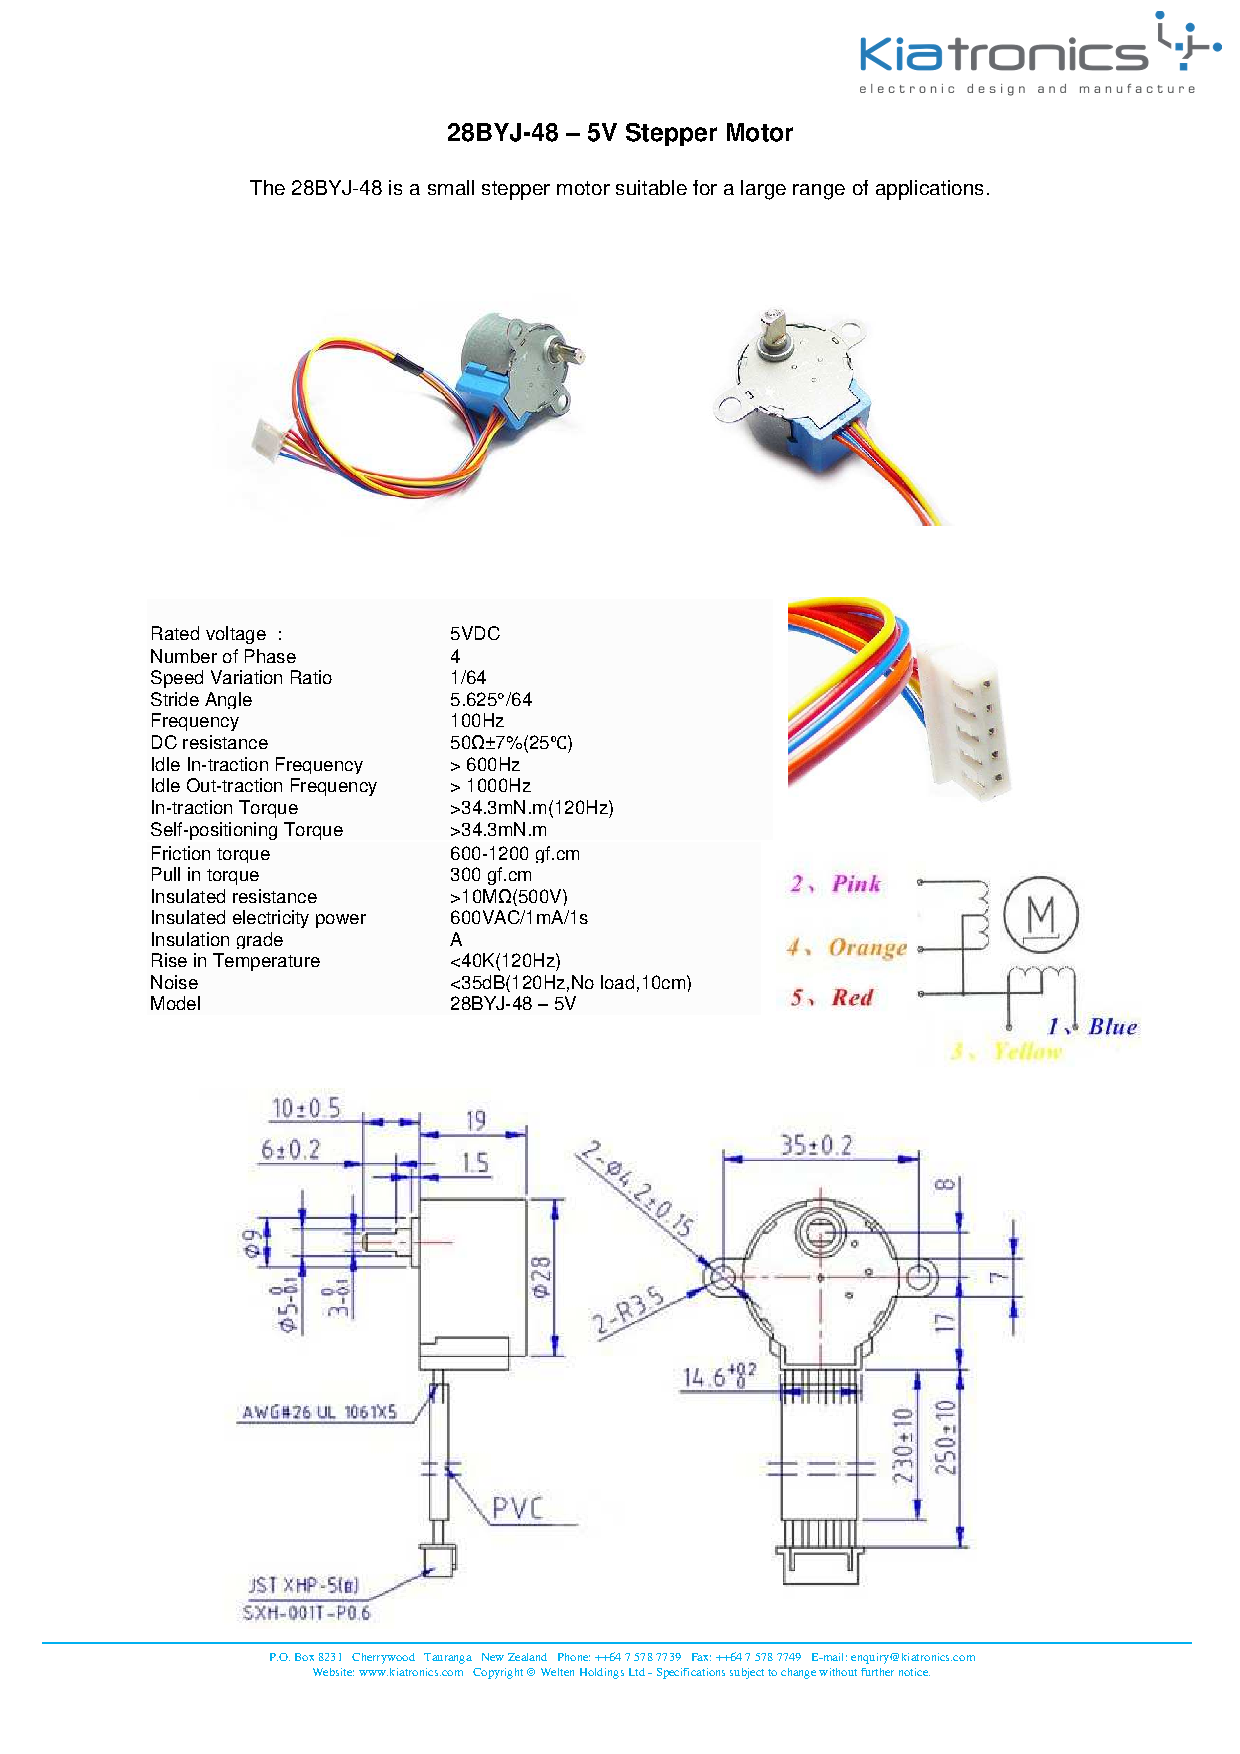
\includepdf[pages={1},width=1.1\linewidth, pagecommand={\thispagestyle{plain}}]{docs/Data_28BYJ-48.pdf}
			\newpage
			\begin{center}
				\vspace*{\fill}
				\centering \Huge Display
				\vspace*{\fill}
			\end{center}				
			\newpage
			\includepdf[pages={5,6,10},width=1.1\linewidth, pagecommand={\thispagestyle{plain}}]{./docs/Data_LCD1602.pdf}
			\newpage
			\begin{center}
				\vspace*{\fill}
				\centering \Huge Operationsverstärker
				\vspace*{\fill}
			\end{center}				
			\newpage
			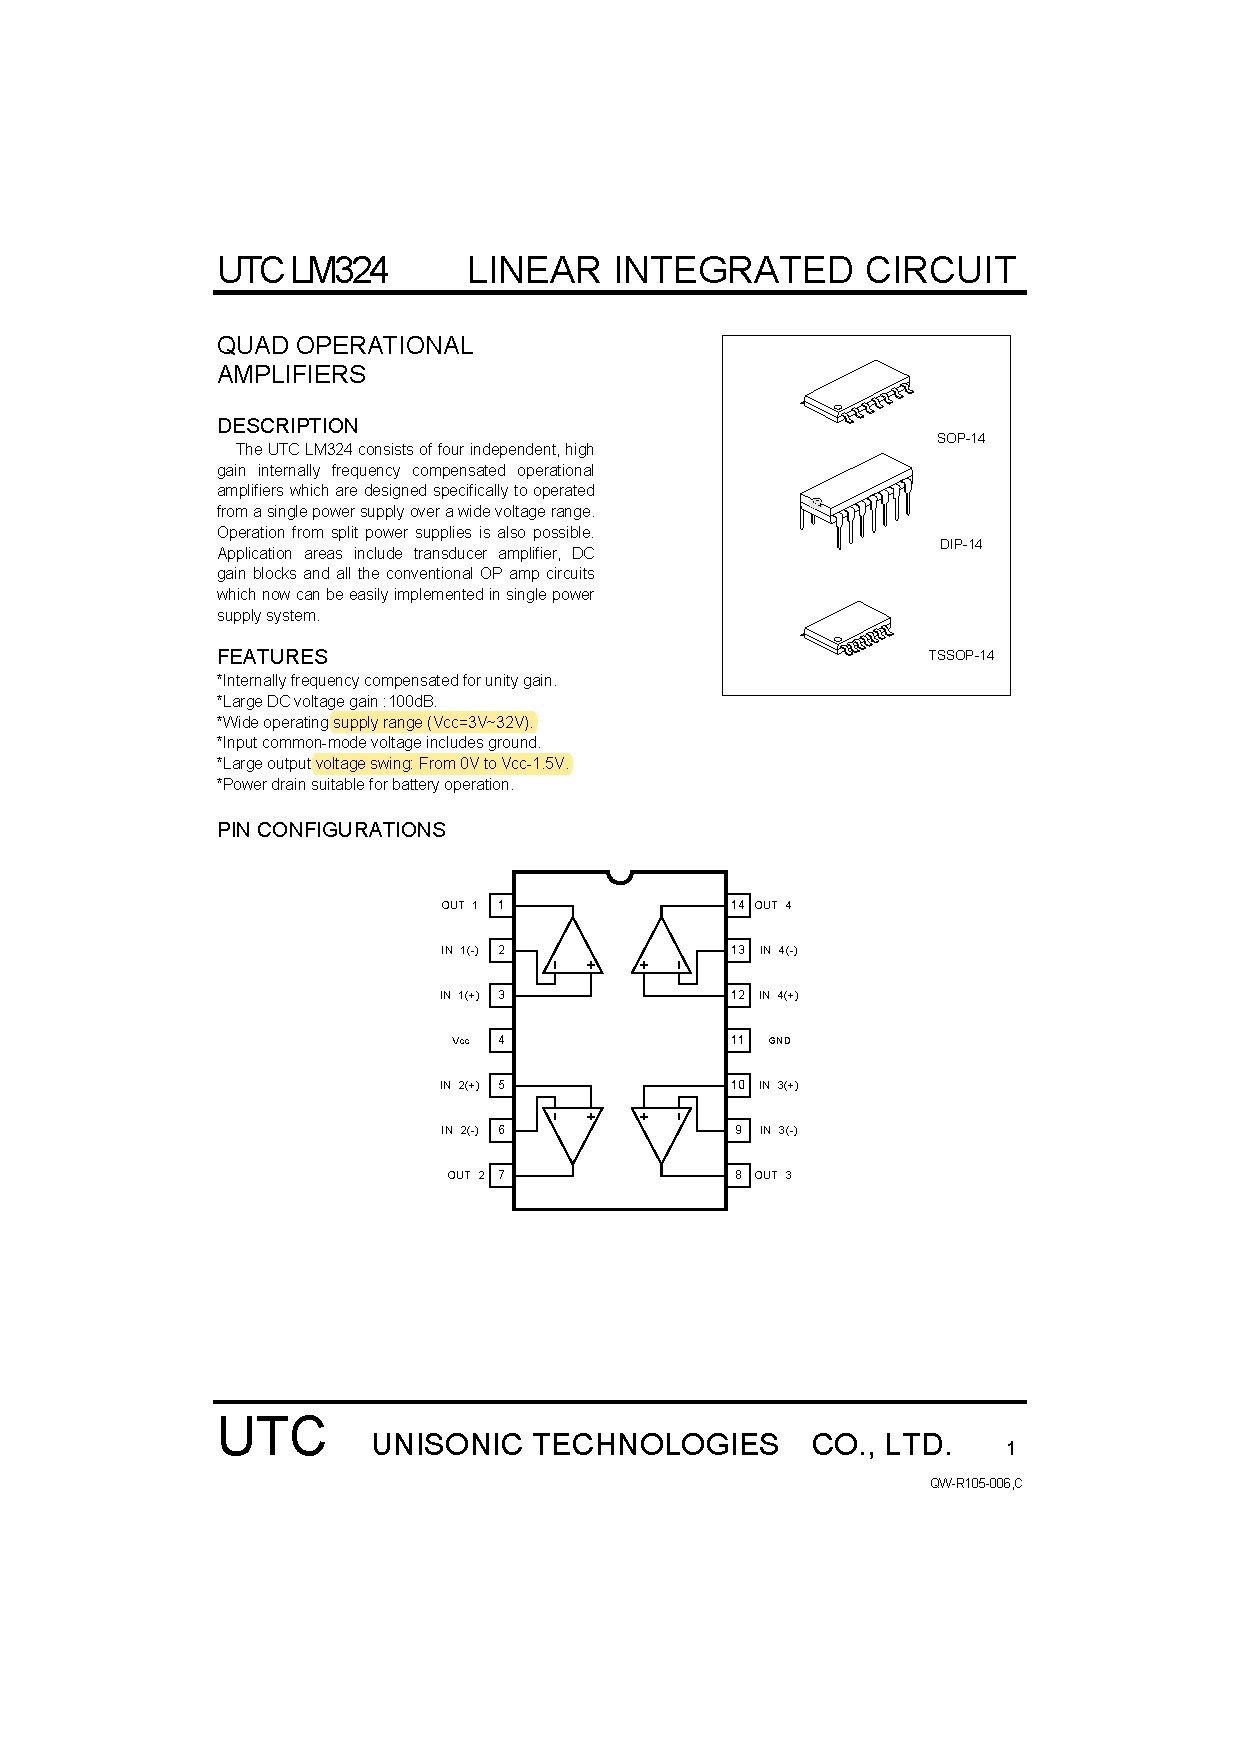
\includepdf[pages={1,3},pagecommand={\thispagestyle{plain}}]{docs/Data_LM324.pdf}
			\newpage
			\begin{center}
				\vspace*{\fill}
				\centering \Huge Darlington-Array
				\vspace*{\fill}
			\end{center}				
			\newpage
			\includepdf[pages={4,5,6},width=1.1\linewidth, pagecommand={\thispagestyle{plain}}]{docs/Data_uln2003.pdf}
			\newpage
			\begin{center}
				\vspace*{\fill}
				\centering \Huge Arduino Nano
				\vspace*{\fill}
			\end{center}				
			\newpage
			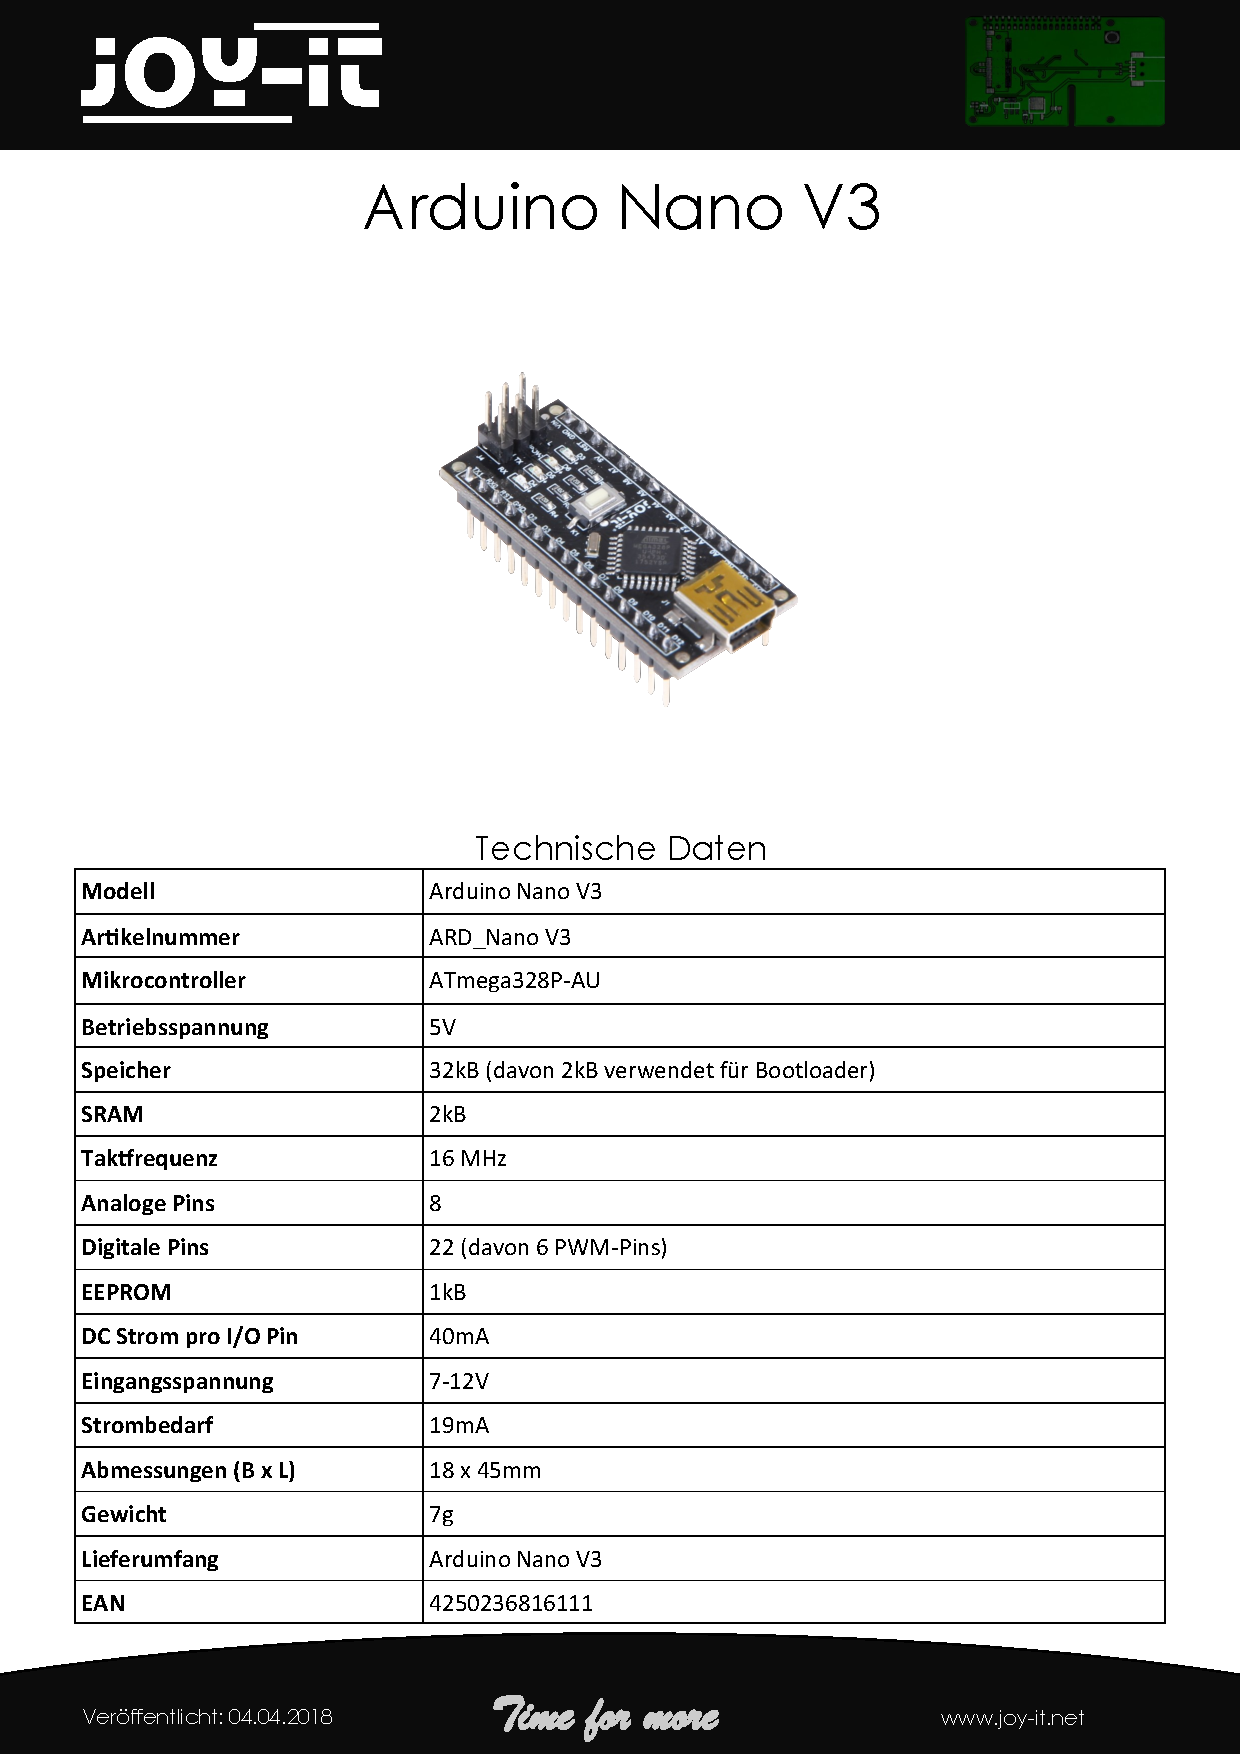
\includepdf[width=1\linewidth, pagecommand={\thispagestyle{plain}}]{./docs/Data_NanoV3_Datenblatt.pdf}
			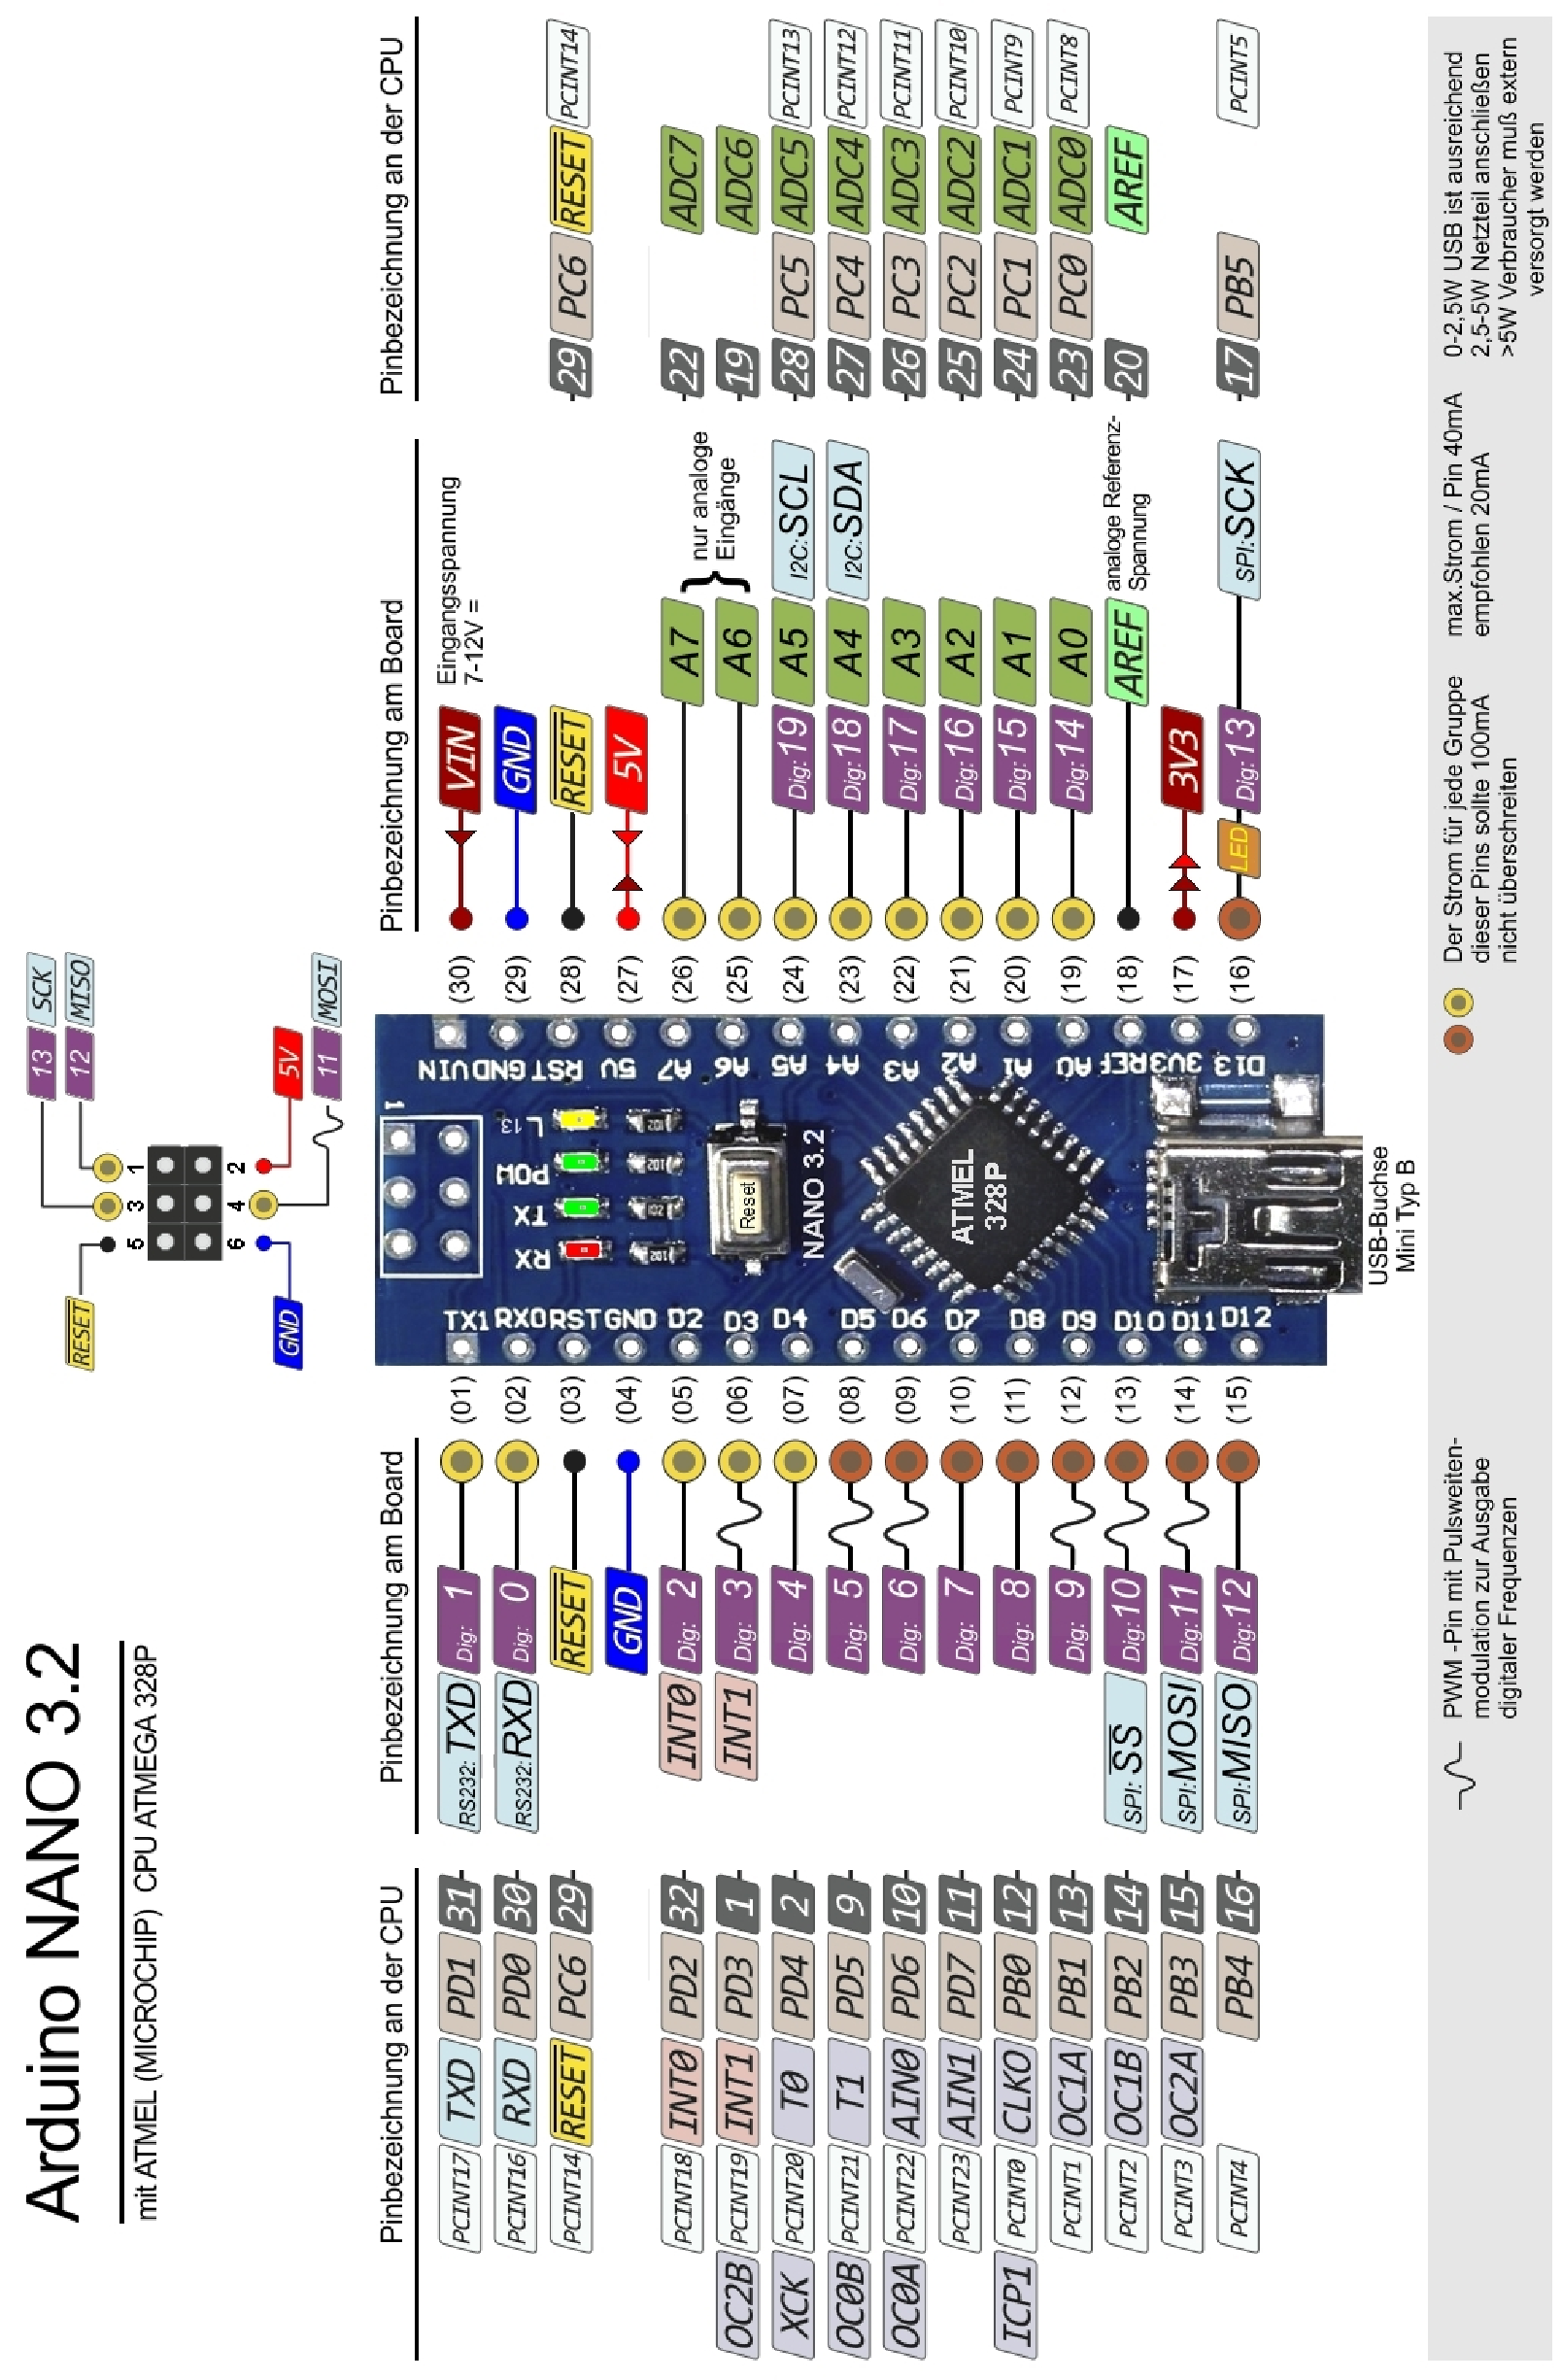
\includepdf[width=0.9\linewidth, pagecommand={\thispagestyle{plain}}]{./docs/Data_NanoV3_pins.pdf}		
		\newpage
		\section{Layouts}
			~
			~
			\begin{figure}[!htbp]
				\centering
				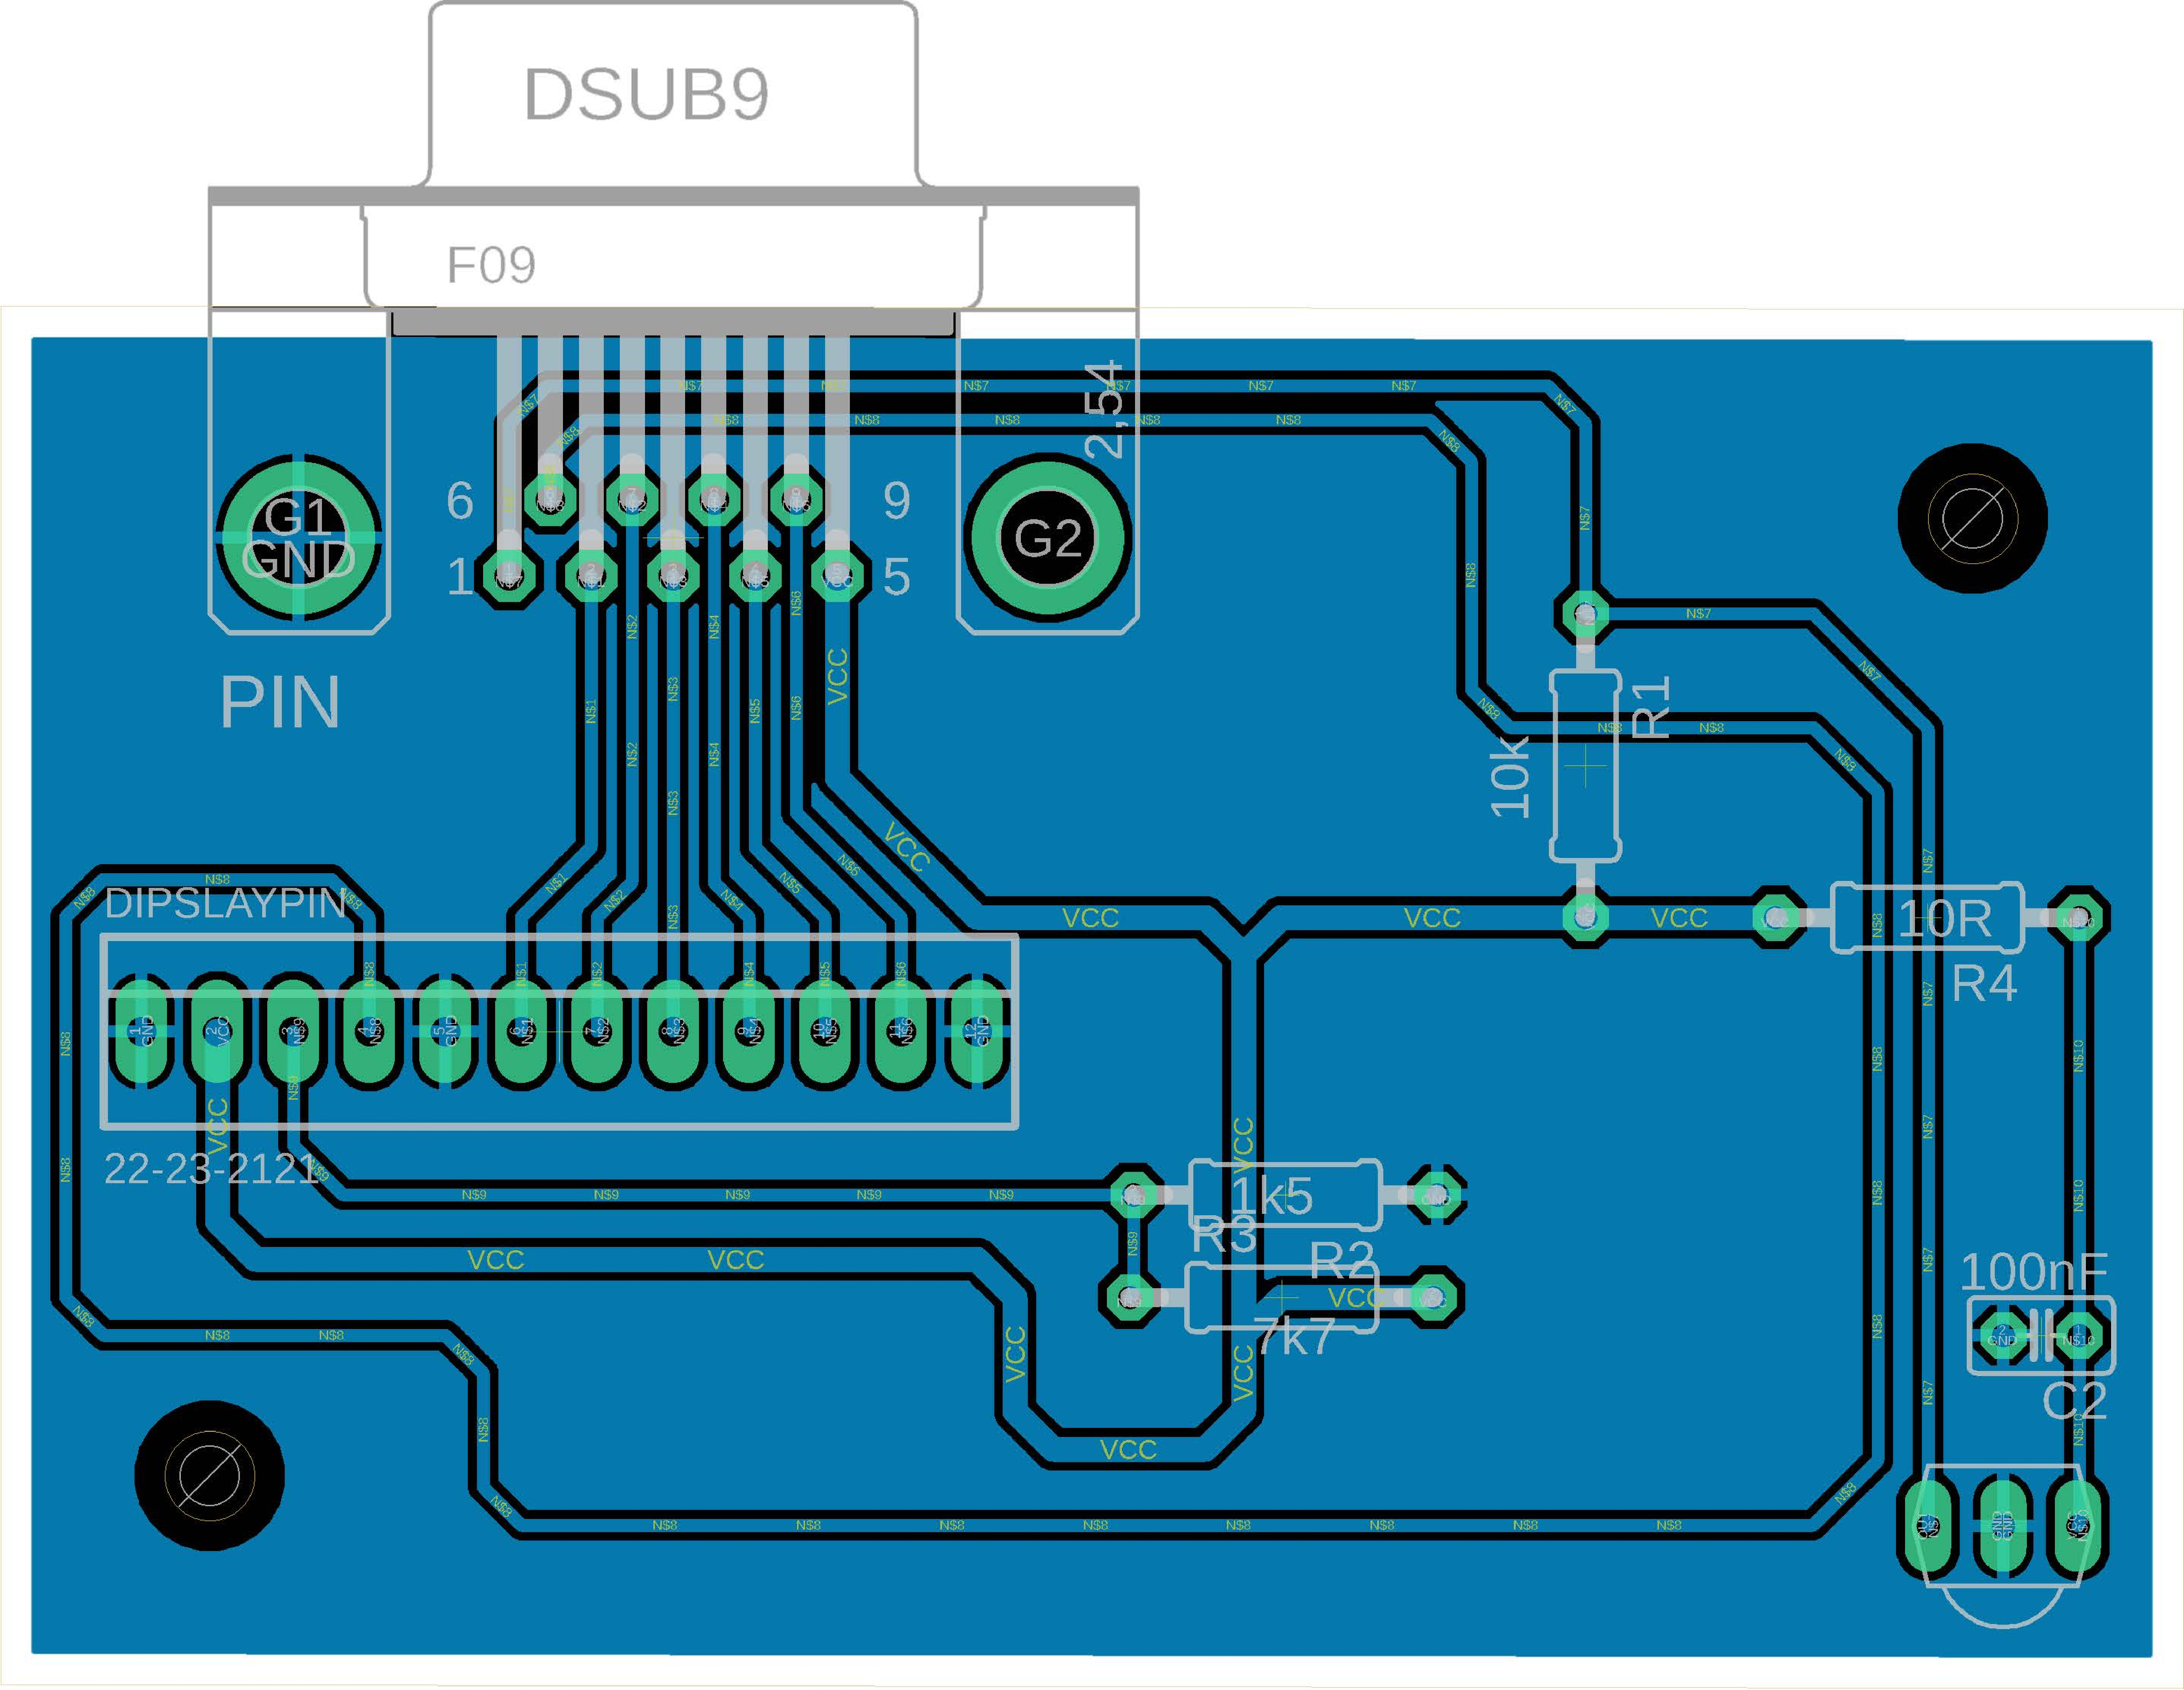
\includegraphics[height=0.9\linewidth ,angle=90]{./docs/Display_LayoutW.pdf}
				\caption{Display-Platine}
			\end{figure}
			\newpage
			~
			~
			~
			\begin{figure}[!htbp]
				\centering
				\includegraphics[height=0.9\linewidth ,angle=90]{./docs/Motor_LayoutW.pdf}
				\caption{Motor-Platine}
			\end{figure}
		\newpage
		\addtocounter{section}{1}
		\addcontentsline{toc}{section}{5.4\hspace{1em}Technische Zeichnungen - Gehäuse}
		\label{sec:TechDraws}
			%Technische Zeichnungen von FreeCAD mit den Abmessungen der Gehäuse.
			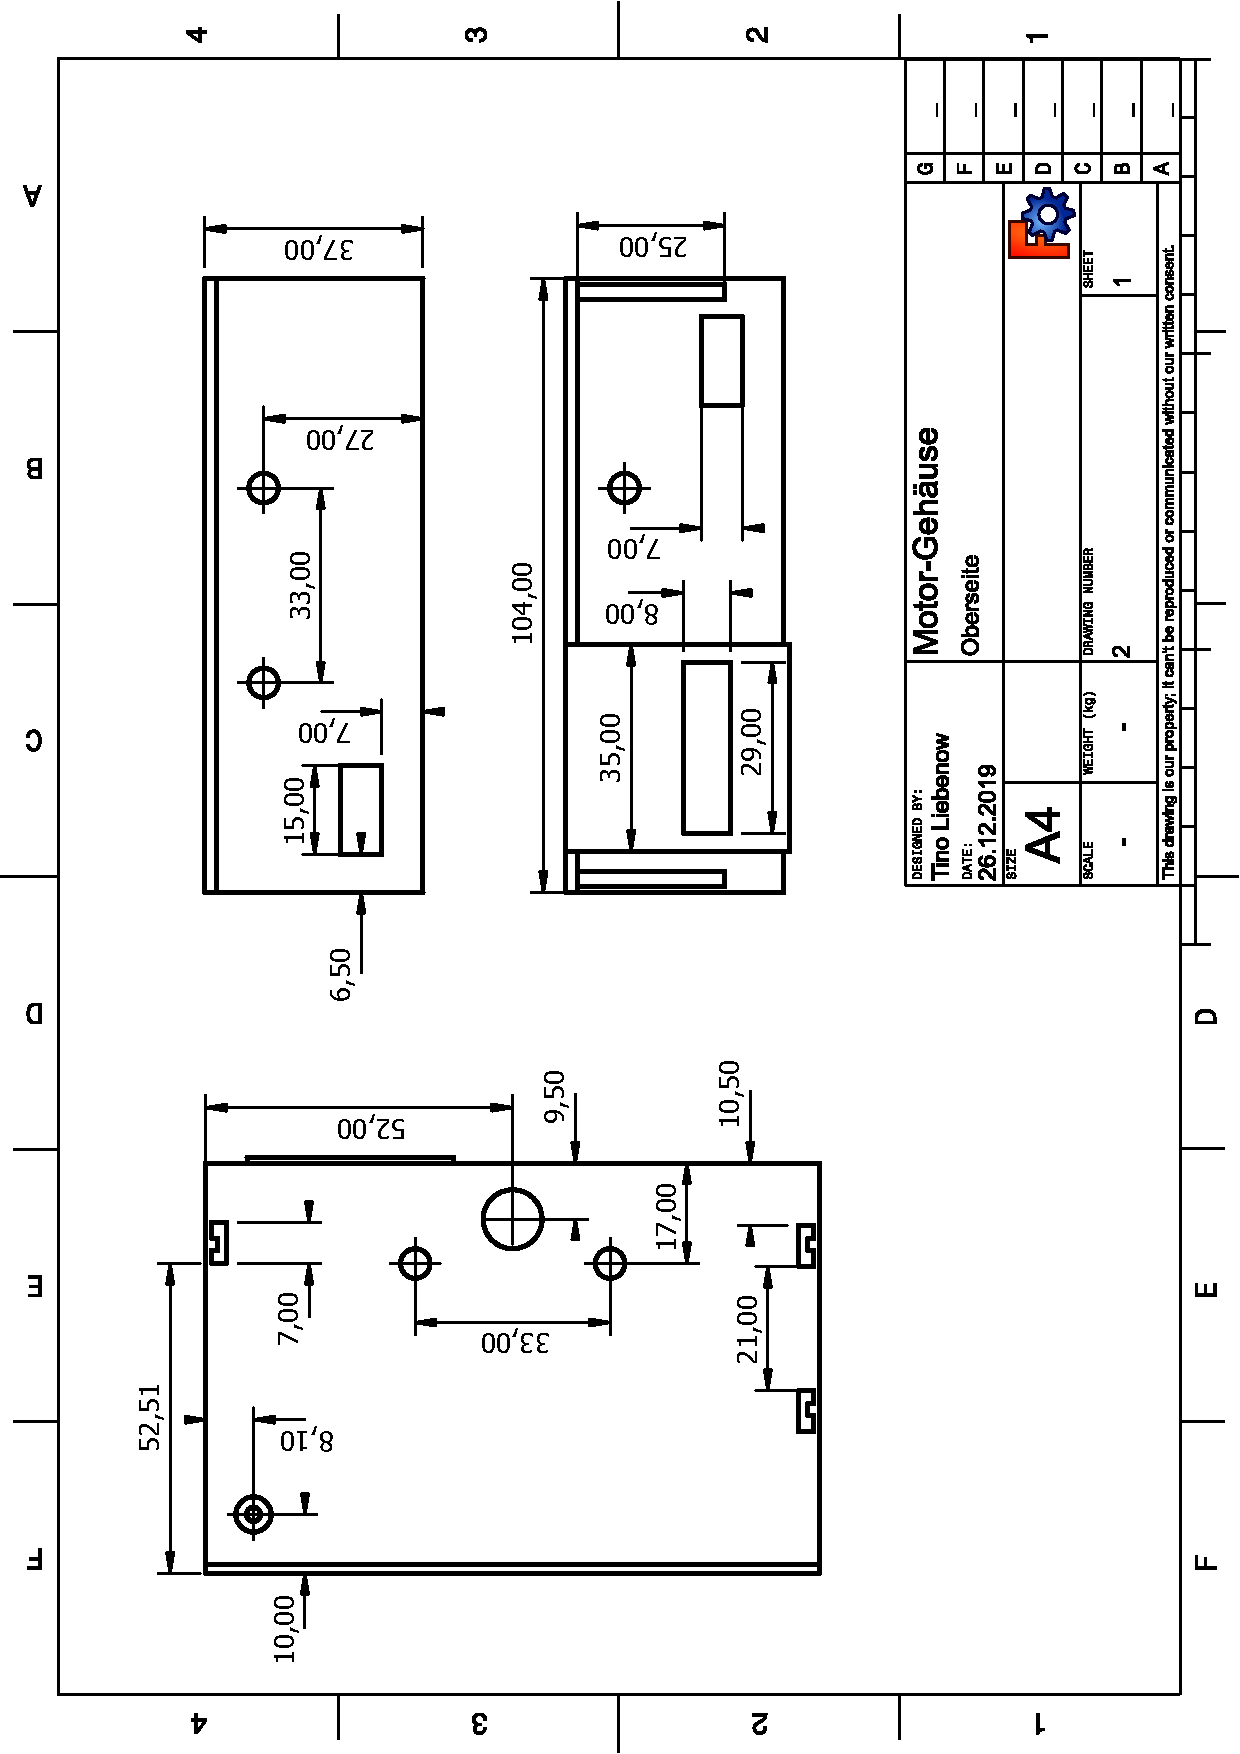
\includepdf[width=1\linewidth, pagecommand={\thispagestyle{plain}}]{./docs/Motor_Case_Oben.pdf}
			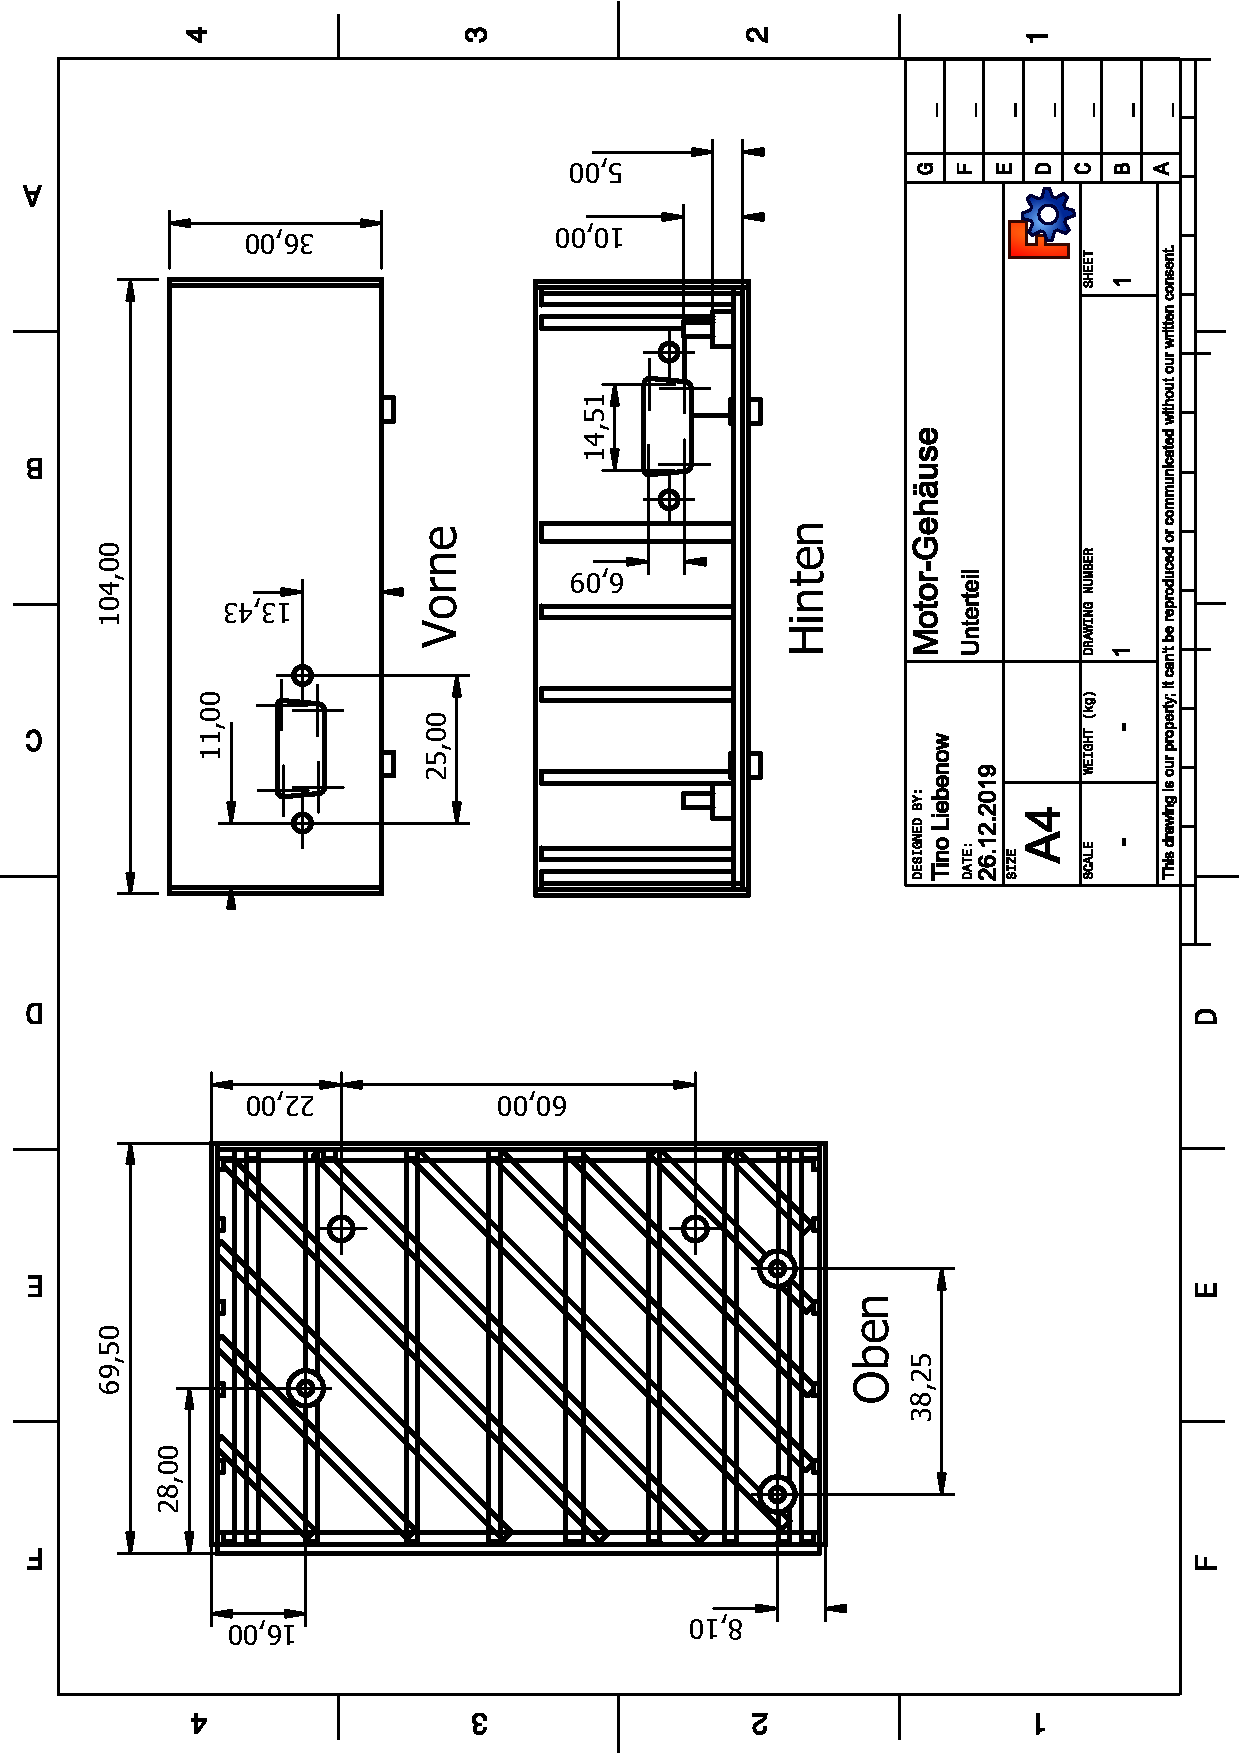
\includepdf[width=1\linewidth, pagecommand={\thispagestyle{plain}}]{./docs/Motor_Case_Unten.pdf}
			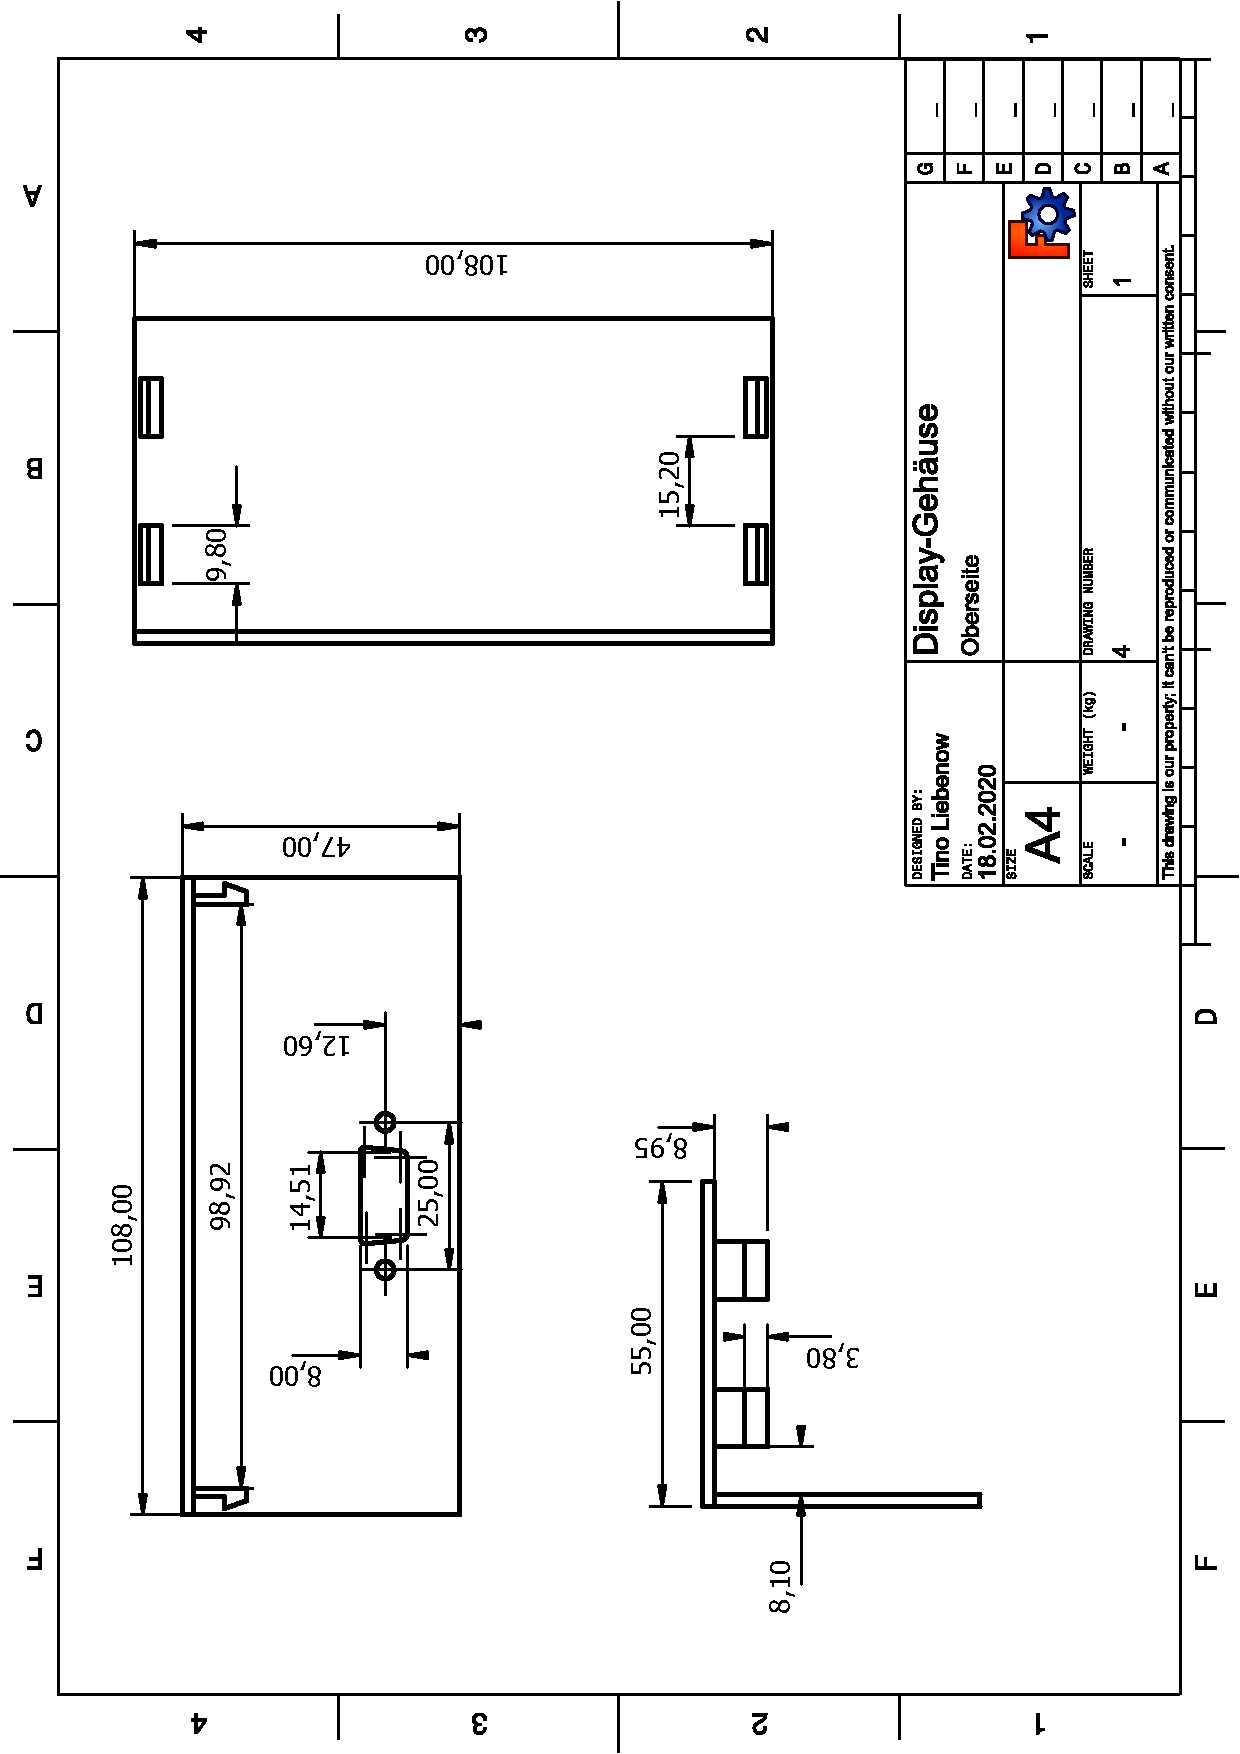
\includepdf[width=1\linewidth, pagecommand={\thispagestyle{plain}}]{./docs/Display_Case_Oben.pdf}
			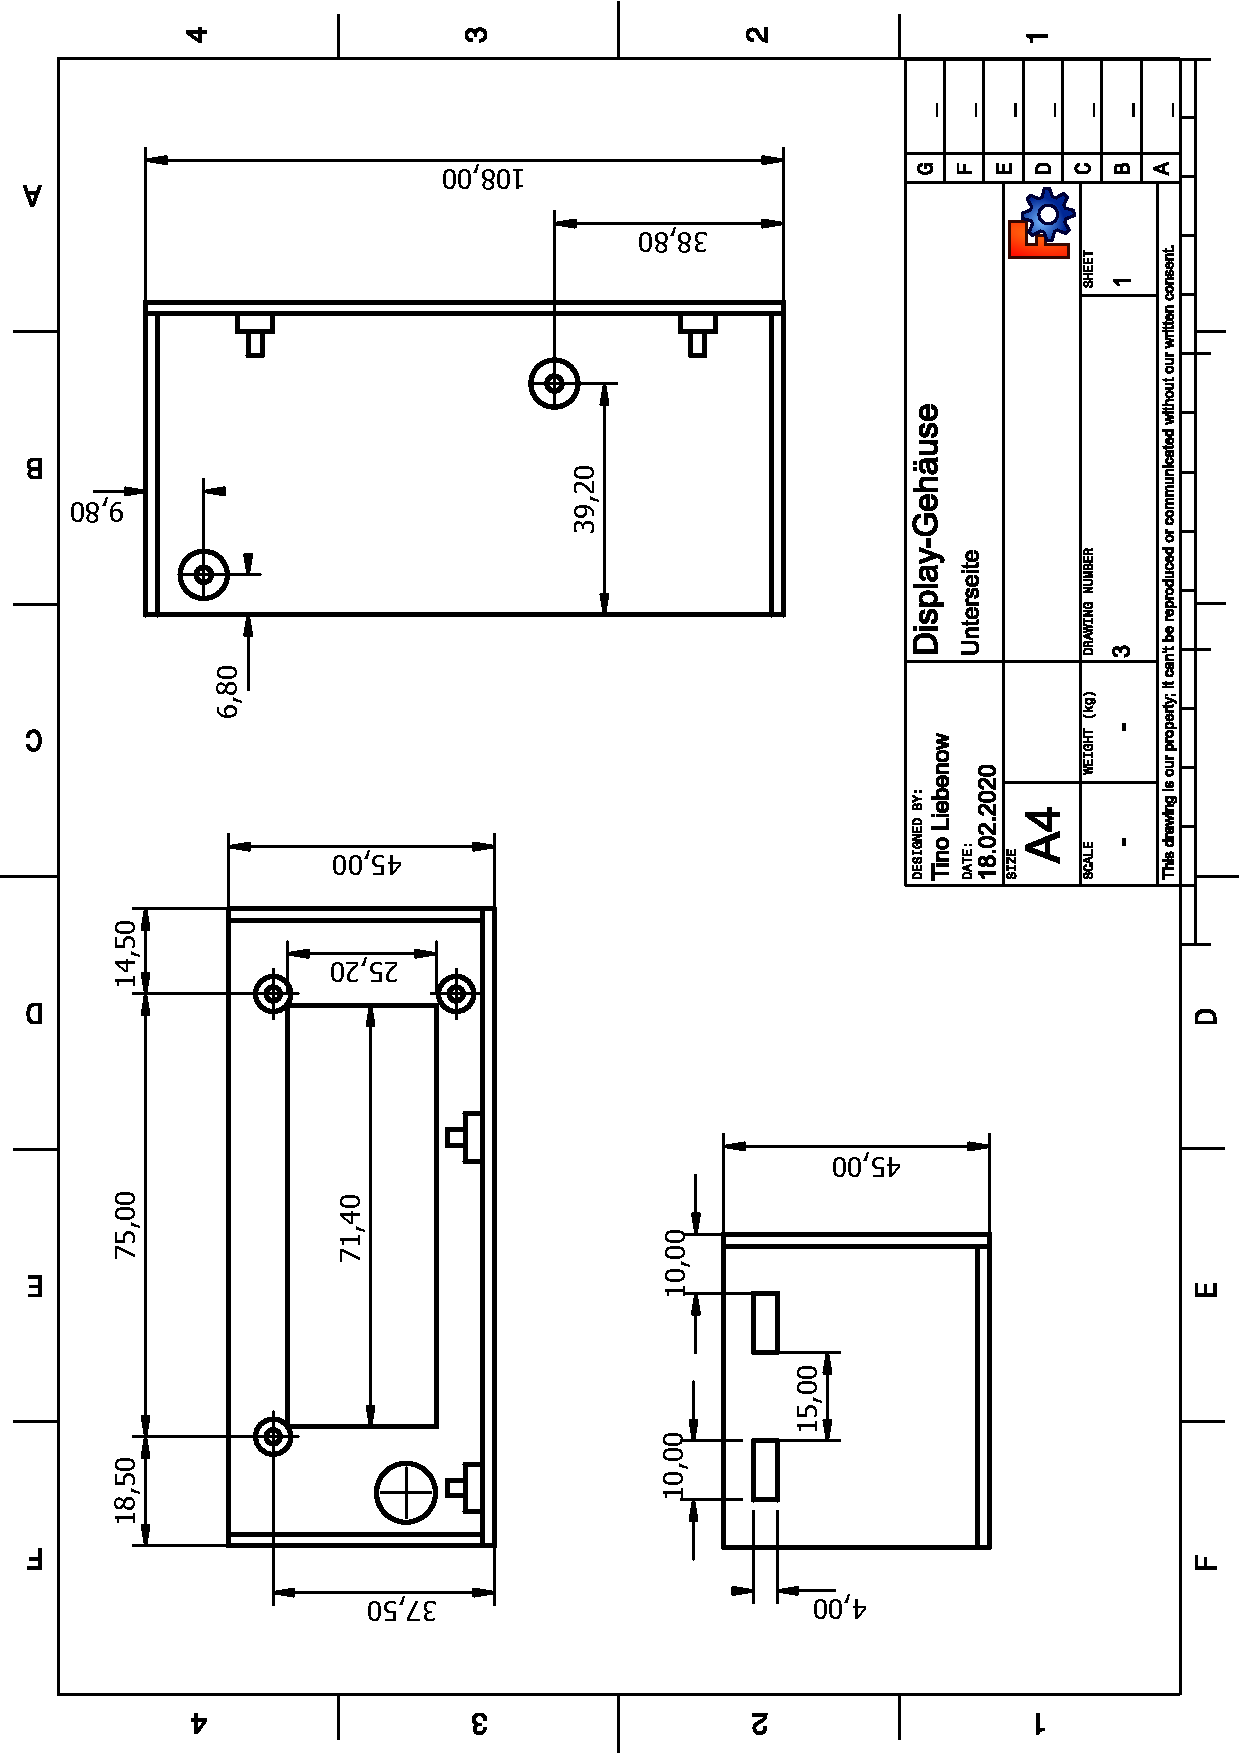
\includepdf[width=1\linewidth, pagecommand={\thispagestyle{plain}}]{./docs/Display_Case_Unten.pdf}
		\section{Quellcode}
		\label{sec:Code}
			Ausschnitte des Quellcodes zur Motorsteuerung:
			\begin{lstlisting}[gobble=28, frame=single, language=C++]
				int arrayDefault[4] = {LOW, LOW, LOW, LOW};
				int outArray[4];
				int stepMatrix[4][4] = {
  				  {HIGH, LOW, LOW, LOW},
  				  {LOW, HIGH, LOW, LOW},
  				  {LOW, LOW, HIGH, LOW},
  				  {LOW, LOW, LOW, HIGH},
				};

				void writeStep(int outArray[4]) {
				  digitalWrite(9, outArray[0]);
				  digitalWrite(10, outArray[1]);
				  digitalWrite(11, outArray[2]);
				  digitalWrite(12, outArray[3]);
				}

				void moveOneStep(bool dir) { //dir = Richtung des Steps
  				  if (currentStep >= 0 || currentStep <= 3) {
    			    	  writeStep(stepMatrix[currentStep]);
  				  } else {
    			    	  writeStep(arrayDefault);
  				  }
  				  (dir == true) ? (currentStep++) : (currentStep--);
  				  if (currentStep > 3) {
    			    	  currentStep = 0;
  				  } else if (currentStep < 0) {
    			    	  currentStep = 3;
  				  }
  				  EEPROM.put(1, currentStep);
				}

				void moveSteps(bool dir, int steps) {
  				  float lowestVoltage = 5.0;
  				  for (int i = 0; i < steps; i++) {
    				  moveOneStep(dir);
    				  float u=currentVoltage();
    				  if (u < lowestVoltage) {
      					  lowestVoltage = u;
    				  }
    				  delay(2);
  				  }
  				  lcd.clear();
  				  uaMin=lowestVoltage;
				}
			\end{lstlisting}
			\newpage
			Auschnitte der Messung und Auswertung der IR-Signale:
			\begin{lstlisting}[gobble=28, frame=single, language=C++]
				void check() {
  				  if (uaMin > 2.8) {
    			  	  impact = false;
  				  } else {
    			  	  Serial.println("ANSCHLAG");
    			  	  impact = true;
  				  }
				}

				float currentVoltage() {
  				  return analogRead(messPinUa) * 5.0 / 1024;
				}

				void motorControl(unsigned long buttonID) {
  				  switch (buttonID) {
    			  	  //Remote pressed "+"
    			  	  case 0xFF02FD:
      					  if (!maxHit) {
        					  moveSteps(true, 1 * 64);
        					  Serial.println(uaMin);
        					  check();
        					  if (!impact) {
          					  volume++;
        					  } else {
          					  lcd.print("STOP");
          					  delay(2000);
          					  lcd.clear();
        					  }
      					  } else {
						  lcd.print("MAX");
      					  }
						EEPROM.put(0, volume);
      					  lastButton = buttonID;
      					  break;

    				  //Remote hold button
    				  case 0xFFFFFFFF:
      					  motorControl(lastButton);
      					  break;
  				  }
				}

			\\end{lstlisting}
	\printbibliography  
\end{document}